%!TEX root = ../template.tex
%%%%%%%%%%%%%%%%%%%%%%%%%%%%%%%%%%%%%%%%%%%%%%%%%%%%%%%%%%%%%%%%%%%%
%% chapter2_SotA.tex
%% NOVA thesis document file
%%
%% Chapter with the State of the Art
%%%%%%%%%%%%%%%%%%%%%%%%%%%%%%%%%%%%%%%%%%%%%%%%%%%%%%%%%%%%%%%%%%%%

\typeout{NT FILE chapter2_SotA.tex}

% \printbibliography[heading=subbibliography, segment=\therefsegment, title={\bibname\ for chapter~\thechapter}]
\glsresetall
\chapter{State of the Art}\label{cha:chapter2_SotA}
% escrever aqui qlq coisa de introduçao:

This chapter focuses on providing a review of the state of the art of the technologies that play a role in an equipement of such complexity as an RTK base station. Afterwards, in a more thorough manner, this can be translated in the study of the technologies employed by the current solution that Beyond Vision offers in the field of precise navigation -- the beRTK\textsuperscript{\textregistered} Base Station.

Starting with the clarification of the operation of different GNSS constellations in Section~\ref{sec:II_gnss}, other different positioning techniques become easier to dissect throughout Section~\ref{sec:II_gnssAug}, which clarifies details about the real-time factor in navigation.
Following that, the current most relevant solutions (i.e. base stations) are addressed and compared in Section~\ref{sec:II_curr_solutions}, along with beRTK\textsuperscript{\textregistered}'s current architecture.

% \textbf{Precision Farming}
% a. Survey every inch of your field
%     Allows detailed survey of every field
% b. Improves productivity and efficiency
%     Reduce time spent on field-walking
% c. Higher resolution of the field areas of interest
%     It is beneficial for immediate identification and GPS tagging
% d. Earlier identification of potential crop issues
%     Use of multispectral sensing technology


    % Começar com:
    % I. o que é uma base station? fazer analogia
    % II. dizer para que e que serve
    % III. onde/no que é que eu vou empregá-la?
    % IV. que tecnologias utiliza?
    % V. explicar cada tecnologia relativamente a base

    % artigos que li:
% a. Experimental Testbed and Methodology for the Assessment of RTK GNSS Receivers Used in Precision Agriculture;

% b. DETERMINATION OF THE POSITION USING RECEIVERS INSTALLED IN UAV

% c. High-Precision/Throughput Growth Measurement of Crops by Drone with Stereo Matching Based on RTK-GNSS and Single Camera

% d. Estimation of the Base Station Position Error in a RTK Receiver Using State Augmentation in a Kalman Filter
% e. Resilient Deployment of Drone Base Stations

% f. Based on a single-base station RTK control survey and precision analysis

% g. Design of an Autonomous drone for IoT deployment analysis

% h. RTK+ System for Precise Navigation in Shadowed Areas

\section{Global Navigation Satellite System}\label{sec:II_gnss}

% enter a NUTSHELL setting of RTK,
UAVs (e.g. drones) are, nowadays, capable of aiding in the most diverse fields, such as search and rescue, delivery, precision farming or even to put on a dazzling light show. Some of these missions require long periods of operation, as well as high positioning precision, and therefore, there might be little to no margin for error, which means that when human variables are introduced in such activites, efficiency is, ultimately, sacrificed. An external aid is required in order for these type of devices to deliver the best possible performances and minimize danger. This can be accomplished via satellite signals. While drones themselves are capable of establishing a link with a GNSS constellation's satellite, the dynamic nature of the former causes a significant latency in the interpretation of the positioning information relayed by the latter. To enhance the precision variable, a stationary equipment known as a base station is capable of fine-tuning the UAV's position in real time, therefore ensuring its intended functions. Such ability is achieved through the use of a specially designed tool: a GNSS receiver.

% Whenever one wishes to know their current location on Earth, a few effortless taps on a smartphone usually prove to be the quickest way to do it; this is often associated with the radionavigational system of GPS (a GNSS itself).
% to conclude that, in order to help tracking their location through the use of satellites, typical smartphones or GPS navigation systems in cars have GNSS receivers, just like a specially designed surveying device.

According to~\cite{novatel_gnss,kaplan_2017}, the best way to address GNSS receivers as a whole is to start by acknowledging its working basis: satellites. While orbiting the Earth, these machines send out signals that are then acknowledged by receivers (hence the name), assisting them on the calculation of their own location on Earth by comparing the received information from other satellites.

% minha parte: METER ISTO NA INTRODUÇÃO DESTA SECÇÃO - GNSS (GERAL)
Through~\cite{fed_rad_plan_2008}, it is possible to understand that, in order to enjoy the perks of assisted navigation, the quality behaviour of a GNSS must be ensured.
A smart approach for that is to analyse the following four performance criteria:

\begin{itemize}
    \item Accuracy: Reminding it should not be confused with precision, this parameter acts as a measure of coherence between the estimated (predicted) and actual position of a vehicle, aircraft, or vessel, at any given time;
    \item Availability: In a percentile manner, this gives the navigator the ability to know the amount of time available to benefit from the services provided by the system, within a certain specified coverage area.
    \item Continuity: Refers, in probabilistic terms, to the ability of the entire system of maintaining all required functions, whilst keeping any interruptions out of question. This ensures smooth operation within a given time interval, assuming the system was fully available at the start of this operational phase;
    \item Integrity: Measuring the trustworthiness of the information supplied by a navigation system, integrity is also able to consistently issue warnings when navigation through the use of the system is not recommended.
\end{itemize}
All of these parameters are defined as a way to rate the performance of a satellite constellation, which helps tracking down any discrepancies or even problems that might make accurate navigation unacceptable.
Their foundation is known as the Required Navigation Performance (RNP) specification, which characterises the imperative performance indicators within a defined airspace. By ensuring the proper conduct of a constellation, the perks of a GNSS for navigation purposes are clear.

Therefore, it is possible to understand that a GNSS comprises a network of satellites that, while continuously orbiting the planet, constantly emit radiofrequency signals carrying information about their current status, position in space and precise time.
This information is achieved through atomic clocks, installed within the satellite itself. Thus, the process unfolds as follows:

\begin{enumerate}
    \item Satellites will start the transmission of their position in real time;
    \item As this happens, the receiver on Earth will be looking for a signal from the satellite, and by the time that signal is received, there will be a delay between transmission and reception, being that radio signals travel at the speed of light ($c$);
    \item Knowing both these timestamps, a GNSS receiver is then able to calculate the difference between the two and determine the time it took to receive the signal;
    \item Lastly, multiplying this calculated time interval by the speed of light, it is then possible to find the distance from the satellite to the receiver.
\end{enumerate}
This process is known as ``trilateration'' and it incorporates the idea that the time ($t$) it takes to receive a signal from a satellite, multiplied by the speed of light ($c$), will equal its distance ($d$) from the surface of the Earth:

\begin{equation}\label{eq:2_1}
    d = v\,t = c\,t\,\medskip
\end{equation}

The signals emitted by satellites propagate in an omnidirectional way, which can be geometrically pictured as an expanding sphere around it -- as it's known from radiation and propagation of electromagnetic waves theory --, meaning the signal will reach the Earth in numerous locations (Figure~\ref{fig:omnidirectional}).
Having another satellite orbiting around Earth, the signal emitted by it will reach the surface at some other particular time. Geometrically, this means that the intersection of the spheres that represent these two signals will correspond to a circle, which limits the extensive list of possible solutions -- note that, however, there is still a large amount --, not allowing yet to have an exact location. Adding a third satellite to this scenario will further limit the possible locations of the receiver, narrowing them down to only two points: one in space and another one down on the surface of the Earth. Knowing that a receiver is down on Earth, by using the latter as a fourth surface, the correct location (in a set of $x$, $y$, $z$ coordinates) can be determined.
% meter imagem word: propagação
\begin{figure}[ht]
	\centering
	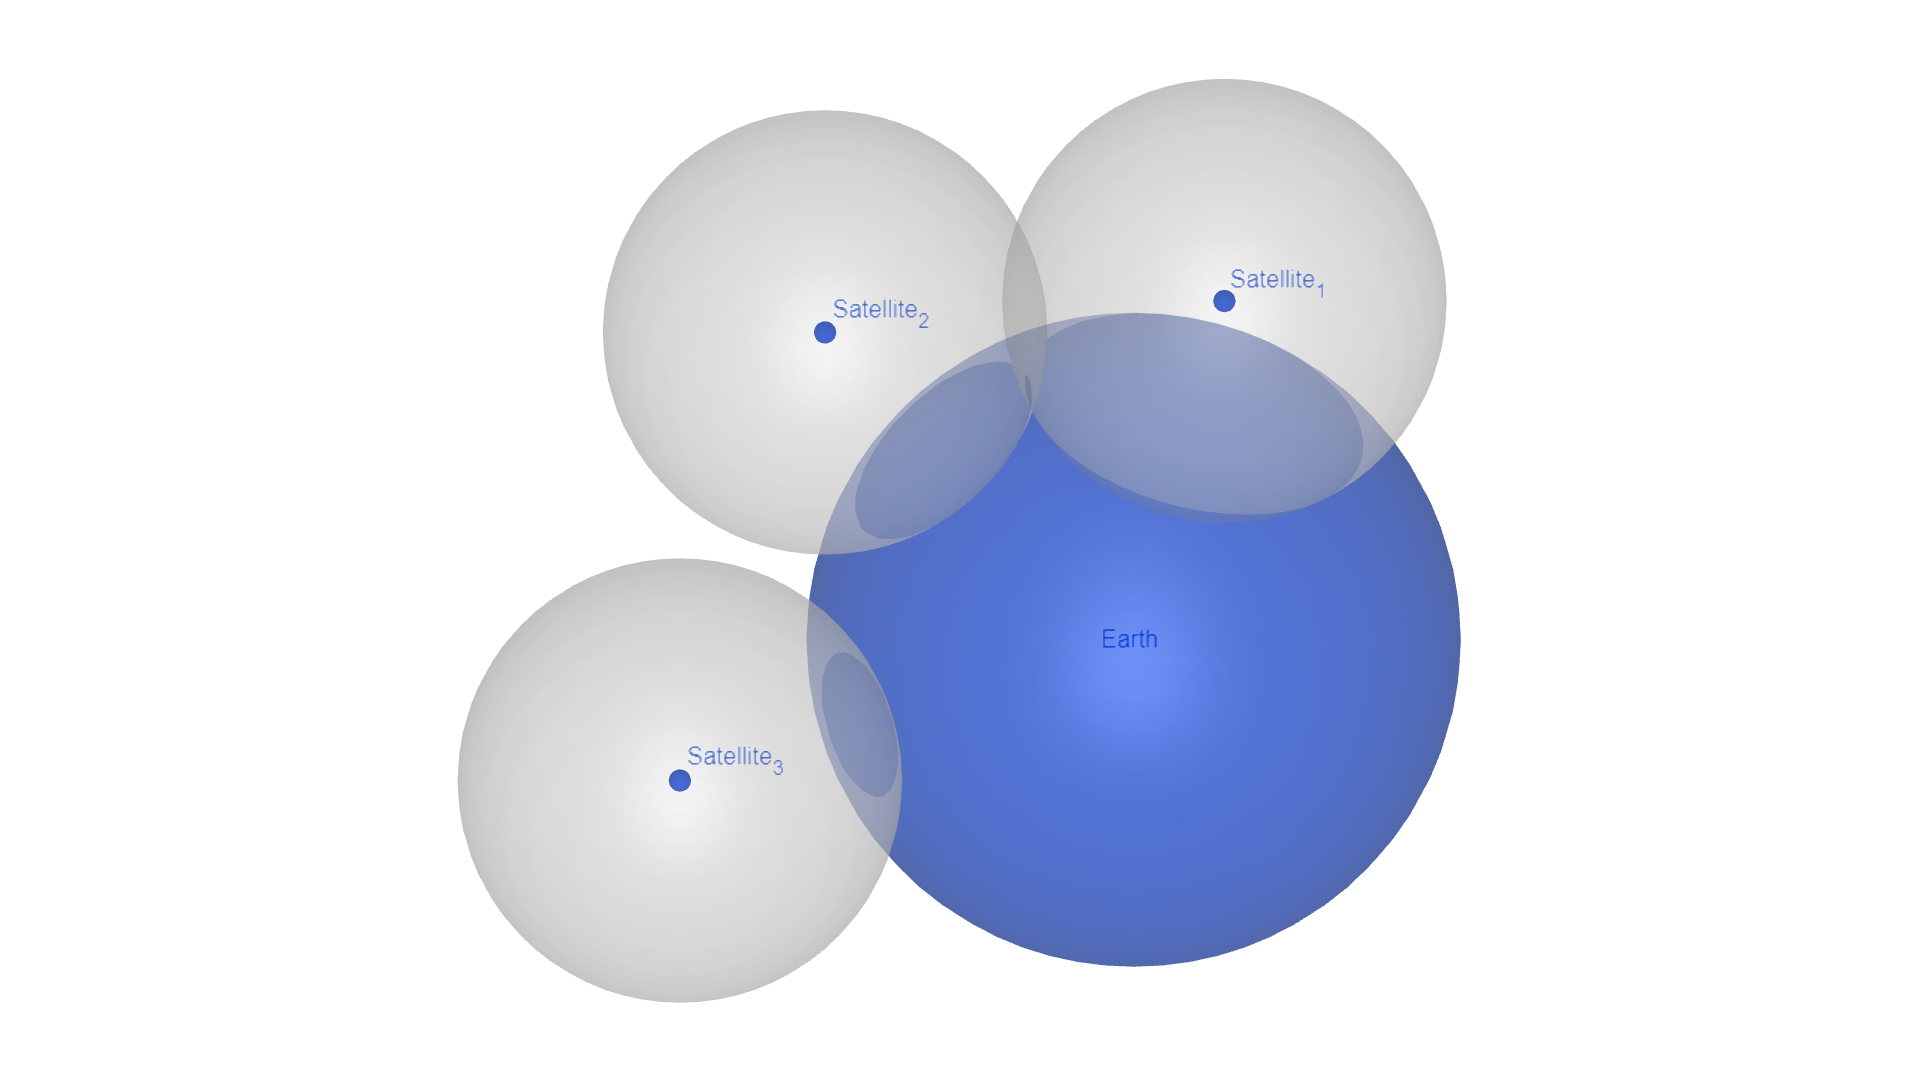
\includegraphics[width=1.0\textwidth]{Chapters/Figures/omnidirectional.png}
	\caption{Propagation of satellite signals.}
	\label{fig:omnidirectional}
\end{figure}
However, just three satellites are not enough for an accurate reading, although in theory this process should be enough. The practical use of trilateration must account with a minimum of four satellites in direct line of sight of any point on the surface of the Earth, in order to synchronise the receiver's clock with the satellites', as well as to better the precision of the solution.
These phenomenons will have a noticeable impact on the timing of the transmitted signals from satellite to receptor, obliterating the intended real-time aspect of navigation. It can be quickly assumed that such aspect will be even more impacted if a variable corresponding to a dynamic nature associated with the receiver exists.
There is, nonetheless, one particular phenomenon able to damage the received signal, resulting in less accurate calculations; it is called \gls{DOP}. This numerical quantity can be measured statistically, while accounting for satellite geometry and location (relative to the receiver) and may, for instance, be impacted by atmospheric or even urban factors.
Logically, it is immediately (and rightfully) assumed that the more satellites there are, the higher the positional accuracy will be for the receiver. For that, to achieve a successful observation, three major segments are necessary, known as the space, control and user segments, as depicted by Figure~\ref{fig:s_c_u_segment}~\cite{gps_USGov,novatel_gnss,ayers_geosystems_2011}.

% meter imagem de predios e sinais afetados
\begin{figure}[ht]
	\centering
	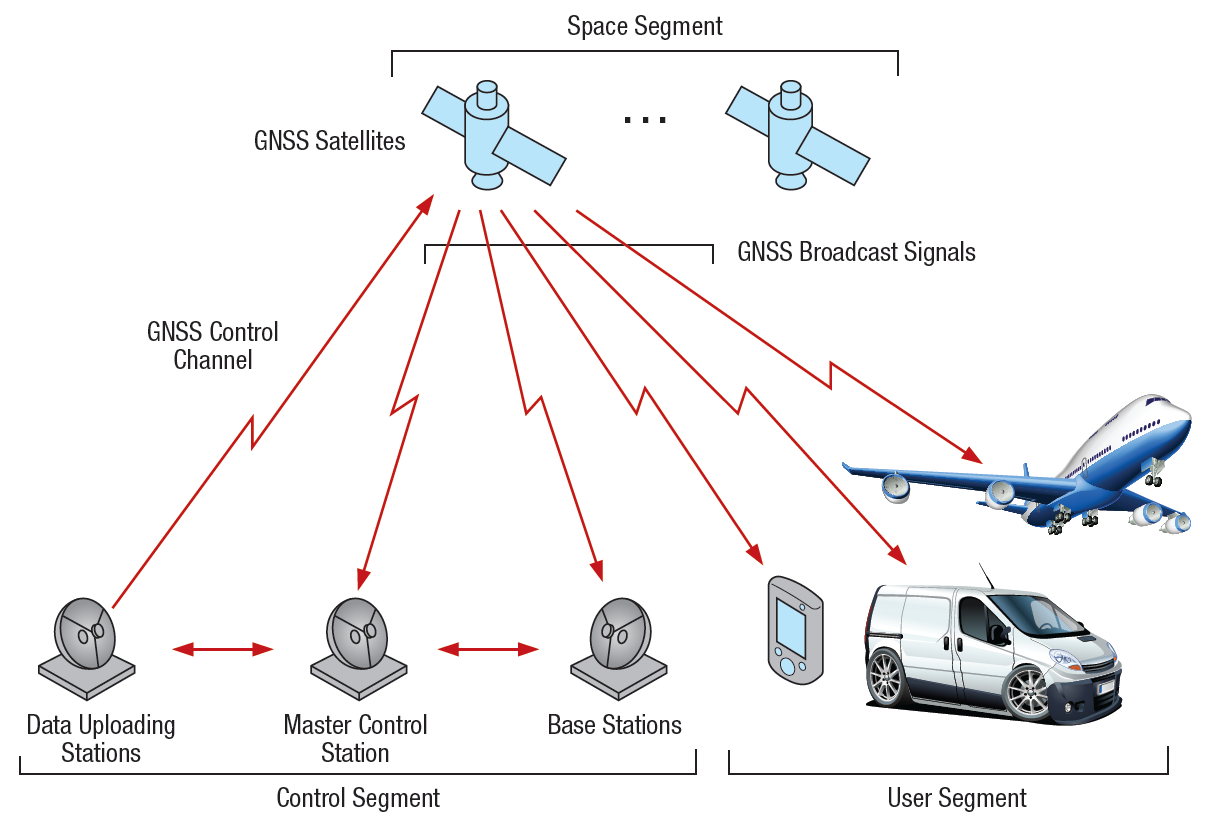
\includegraphics[width=1.0\textwidth]{Chapters/Figures/s_c_u_segment.png}
	\caption{GNSS segments (adapted from~\cite{novatel_gnss}).}
	\label{fig:s_c_u_segment}
\end{figure}

\subsection{Space Segment}\label{sec:II_gnss_space_seg}

The space segment corresponds to the GNSS satellites. All of these follow a certain orbital path thousands of kilometers above the Earth's surface, aiming to assist in the precise location of GNSS-enabled devices on the ground.
Different nations around the world have various satellite networks, with GPS being the most widely known GNSS of all. Developed and established by the United States Department of Defense near the end of the 1970s, this network relies on a constellation made up of a total of 31 satellites, on which the U.S. government works to maintain constant operability of a minimum of 24, 95\% of the time, to guarantee global coverage~\cite{gps_USGov}.
Upon its the introduction to civilian use, the desire to cover an even larger portion of the globe only grew, which led to the development of other GNSSs that, together with the already existing GPS, could improve navigational accuracy. Thus, there are currently four global satellite arrangements that make world navigation and precise positioning possible, described in Table~\ref{tab:5_GNSSs}.
Additionally, there are also two extra systems that were developed to provide regional coverage, NavIC (from India) and QZSS (from Japan).

% \begin{itemize}
%     \item NavIC (India):
%     % Planned to be made up of seven satellites, this Regional Navigation Satellite System was developed by India to grant regional coverage (hence the (outdated) name IRNSS) to India and its neighbouring area.
%     % As a result of the launch of the constellation's last satellite in 2016, the IRNSS title was changed to Navigation Indian Constellation (NavIC), by India's Prime Minister Narendra Modi~\cite{navic_news_2016};
%     \item QZSS (Japan):
%     % Working as another regional navigation satellite system, the development of the Quasi-Zenith Satellite System was accredited by the Japanese government in order to ensure service to Japan, as well as the Asia-Oceania region and consists of four satellites.
%     % However, this constellation limits accuracy in its standalone (also known as single-point positioning) mode, which means it functions as GPS augmentation service\footnote{GNSS augmentation will be covered in more detail in Section~\ref{sec:II_gnssAug}.} by synchronisation of clocks use of same frequencies, allowing the use of this system's machinery as extra GPS satellites.
% \end{itemize}

% table:-----------------------------
\begingroup
\begin{table}[h]
	\caption{Global satellite positioning systems.}
	\label{tab:5_GNSSs}
	\centering%@{}l@{}@{}c@{}@{}c@{}@{}c@{}@{}c@{}
    % \setlength{\tabcolsep}{10pt} % Default value: 6pt
    % \renewcommand{\arraystretch}{1.5} % Default value: 1
	\begin{tabular}{lccccc}
        \toprule
        \multicolumn{2}{c}{\multirow{2}*{\textbf{Constellation}}} & \multirow{2}*{\textbf{Satellites}} & \textbf{Orbital} & \textbf{Orbital}     & \textbf{Orbit} \\
        \multicolumn{2}{c}{}                                      &                                    & \textbf{Planes}  & \textbf{Inclination} & \textbf{Radius} \\
        \midrule

        \multirow{3}*{
\includegraphics[height=1cm]{Chapters/Figures/flags/usa.png}}&\multirow{3}*{GPS} &  &  &  & \\
        \multirow{3}*{}   &{}             & 27 + 4 (spares) & 6 & 55 degrees & $20,200$km \\
        \multirow{3}*{}   &{}          & & & & \\

        \midrule

        \multirow{3}*{
\includegraphics[height=1cm]{Chapters/Figures/flags/Russia.png}}&\multirow{3}*{GLONASS} &  &  &  & \\
        \multirow{3}*{}   &{}             & 24 + 3 (spares) & 3 & 64.8 degrees & $19,140$km \\
        \multirow{3}*{}   &{}          & & & & \\

        \midrule

        \multirow{3}*{
\includegraphics[height=1cm]{Chapters/Figures/flags/Europe.png}}&\multirow{3}*{Galileo} &  &  &  & \\
        \multirow{3}*{}   &{}             & 27 + 3 (spares) & 3 & 56 degrees & $23,222$km \\
        \multirow{3}*{}   &{}          & & & & \\

        \midrule
        \multirow{3}*{
\includegraphics[height=1cm]{Chapters/Figures/flags/China.png}}&\multirow{3}*{BeiDou} & 5 GEO & --- & --- & $35,787$km \\
        \multirow{3}*{}   &{}             & 3 IGSO & --- & 55 degrees & $35,787$km \\
        \multirow{3}*{}   &{}          & 27 MEO & 3 & 55 degrees & $21,525$km \\
        \bottomrule
    \end{tabular}
\end{table}
\endgroup
% não dá para meter \footnote{Geostationary orbit.}
% não dá para meter \footnote{Inclined geosynchronous orbit.}
% não dá para meter \footnote{Medium Earth orbit.}

Every constellation follows the same purpose of providing services of:

\begin{itemize}
    \item Positioning: Refers to the ability of determining one's location and orientation in an accurate and precise manner, either two-dimensionally or three-dimensionally (whenever necessary), taking a standard reference geodetic system (e.g. World Geodetic System 1984, or WGS84);
    \item Navigation: Enables the determination of the current position, as well as the application of course, orientation and velocity corrections in order to achieve a desired position (relative or absolute) at any location in the world, from subsurface to surface and from surface to space;
    \item Timing: Also encompassing time transfer, timing refers to the ability of acquiring the exact and precise time from a certain standard (in this case Coordinated Universal Time, or UTC), as well as maintain it, anywhere in the world and within timeliness parameters defined by the user.
\end{itemize}
These are known as \gls{PNT} services~\cite{pnt_2017}.
A good example of the use of this type of data is the GPS system, which is a result of the use of PNT data together with information from maps, as well as from other sources (e.g. meteorological data, traffic, etc.).

Therefore, the space segment essentially focuses on accurately covering every point on Earth's surface, something which engineers work on to improve every day, whether it being with precision tweaks to the satellites' atomic clocks or even launching new ones to further complement an existing GNSSs~\cite{euspa_news_2022}. This means that all constellations are able to complement each other, and by being used globally, the location accuracy at any given time is increased.

\subsection{Control Segment}\label{sec:II_gnss_control_seg}

Each satellite's status -- specifically, its ``health'', position (current and expected), velocity and timing -- is recorded by an internal orbital pattern known as \gls{ephemeris}. Such data is, in turn, included within the transmitted signals. The control segment is found on Earth, at a stationary location, and its control element is used to correct any errors coming from the satellites, being that the more satellites that can be observed in the control segment, the greater the probability of an error to be detected and corrected, thus increasing accuracy in the user segment.

A good example for the control segment is, precisely, a base station: by installing a GNSS receiver at a fixed location, it will continuously collect data from the satellites, as well as any changes or discrepancies in the readings, which can then be corrected later and transferred to the user segment. Nowadays, there are long-term reference stations that are mounted and freely accessible, which eliminates the need for two receivers; having a base and rover together can be too much equipment in some situations and therefore result in larger financial costs.
In order to solve this, the rover receiver just needs to be connected to some kind of frame of reference, which will be the control segment used to complete the solution (this could be, for example, an NTRIP\footnote{NTRIP will be covered in more detail in Section~\ref{sec:II_networkedRTK_ntrip}.} network).
This type of references are generally found in heavily populated areas; anywhere that is more rural or not really connected to society, they may not be available, so the need to have two receivers in order to complete the three segments will inevitably be felt.

It should be noted that one of this segment's tasks lies in the monitoring of satellites, i.e. the regular adjustment of trajectory and time information, in order to keep all the transmitted information highly accurate.

\subsection{User Segment}\label{sec:II_gnss_user_seg}

The user segment includes smartphones, rovers and anything that has a GNSS receiver installed It is the end result and refers to what needs to be measured (i.e. the location to find). The other two segments act only as a means of helping reach a more precise position for the user segment.
As we try to find the location of a point in a given \gls{geodetic_datum} or coordinate system, regardless of what is being done, taking a survey is about ensuring that all data collected is accurate, and any correction elements used are fully understood.

\subsection{Satellite Communication}\label{sec:II_gnss_comm}

As previously affirmed, GNSS satellites communicate with receivers through electromagnetic signals that propagate omnidirectionally. These machines are designed to continuously orbit along their respective trajectories, and therefore the signals transmitted might run into problems while on their way to Earth, which can occur due to atmospheric reasons or even while the receiver is blocked by something such as a building, for example. An affected signal reaching a receiver will result in a poor reading precision. Table~\ref{tab:GNSS_sys_errors} shows the typical errors intrinsic to the GNSS system.

% typical errors: ATENÇÃO À POSIÇÃO DA TABELA!!
\begingroup
\begin{table}[h]
	\caption{Typical GNSS system errors (adapted from~\cite{novatel_gnss}).}
	\label{tab:GNSS_sys_errors}
	\centering%@{}l@{}@{}c@{}@{}c@{}@{}c@{}@{}c@{}
    % \setlength{\tabcolsep}{10pt} % Default value: 6pt
    % \renewcommand{\arraystretch}{1.5} % Default value: 1
	\begin{tabular}{lc}
        \toprule
        \textbf{Source} & \textbf{Error range} \\
        \midrule
        Satellite clocks & $\pm 2.0$ m \\
        \midrule
        Orbit errors & $\pm 2.5$ m \\
        \midrule
        Ionospheric delays & $\pm 5.0$ m \\
        \midrule
        Tropospheric delays & $\pm 0.5$ m \\
        \midrule
        Receiver noise & $\pm 0.3$ m \\
        \midrule
        Multipath & $\pm 1.0$ m \\
        \bottomrule
    \end{tabular}
\end{table}
\endgroup

The communication process can be characterised through an intricate set of terms such as \gls{pseudorandom}, \gls{correlation} and code division multiple access (CDMA). According to~\cite{novatel_gnss}, this categorizes the GNSS positioning technique as ``code-based'', meaning the receiver operates through pseudorandom noise codes (or PRN codes) transmitted by four or more satellites, correlating with these in order to determine time and position.

Theoretically, information should be able to flow smoothly, however, due to the aforementioned dilution of precision, signals may be affected while travelling through the atmosphere;
the propagation signal can be affected when it passes through the ionosphere (a layer located roughly 50-1,000 km above Earth's surface) or the troposphere (located about 8-14.5 km above the surface), which correspond to the upper and lower zones of the atmosphere, respectively. These effects depend significantly on frequency, so it is worth noting that signals can be compromised by negative effects such as reflection and even absorption, scintillation, Faraday rotation and bandwidth decoherence\footnote{For a clearer definition of the negative effects, refer to~\cite{ieee_terms_1997}.}~\cite{au_gov_satell}. Considering these problems, GPS was designed to operate in frequencies within the interval of 1 to 2 GHz, which corresponds to a section of the radio spectrum known as the L-band, as represented by Figure~\ref{fig:gps_bands} (which shows the frequency bands used in GPS communication, known as the L1, L2 and L5 frequencies).
% meter/fazer figura das frequencias do GPS:
\begin{figure}[ht]
	\centering
	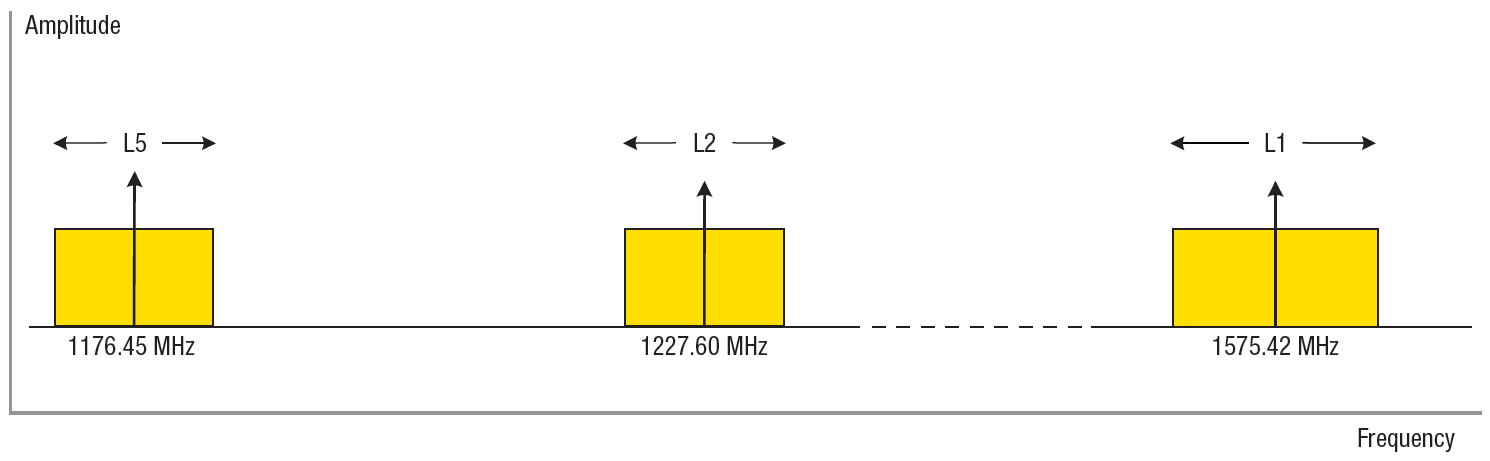
\includegraphics[width=1.0\textwidth]{Chapters/Figures/gps_bands.png}
	\caption{GPS frequency bands (adapted from~\cite{novatel_gnss}).}
	\label{fig:gps_bands}
\end{figure}

This band solves a great part of the stated problems due to its high frequencies, as it simplifies antenna design and lowers the impact of ionospheric delay.

% razões 1: MUDAR
% Simplification of antenna design. If the frequency had been much higher, user antennas may have had to be a bit more complex.
% - Ionospheric delay is more significant at lower frequencies.
% - Except through a vacuum, the speed of light is lower at lower frequencies
% - The coding scheme requires a high bandwidth, which was not available in every frequency band.
% - The frequency band was chosen to minimize the effect that weather has on GPS signal propagation.

% razões 2: MUDAR
% L1 transmits a navigation message, the coarse acquisition C/A code (freely available to the public) and an encrypted precision (P) code, called the P(Y) code (restricted access). The navigation message is a low bit rate message that includes the following information:
% - GPS date and time.
% - Satellite status and health. If the satellite is having problems or its orbit is being adjusted, it will not be usable. When this happens, the satellite will transmit the out-of-service message.
% - Satellite ephemeris data, which allows the receiver to calculate the satellite's position. This information is accurate to many, many decimal places. Receivers can determine exactly where the satellite was when it transmitted its time.
% - Almanac, which contains information and status for all GPS satellites, so receivers know which satellites are available for tracking. On start up, a receiver will recover this "almanac".
% The almanac consists of coarse orbit and status information for each satellite in the constellation.

% The P(Y) code is for military use.

% GPS. The L2 frequency transmits the P(Y) code and, on newer GPS satellites, it also transmits the C/A code (referred to as L2C), providing a second publicly available code to civilian users.

\subsubsection{Signal Propagation}\label{sec:II_gnss_comm_propag}

% As mentioned earlier, the atmosphere has a considerable impact on the transmission of signals from GNSS satellites, the layer that most influences transmissions being the ionosphere, taking into account that this layer is responsible, as its name implies, for the ionization of the parts upper atmosphere of Earth. The interaction of the resulting free electrons with the propagating electromagnetic waves gives rise to transmission delays, these delays depending on the frequency at which the signal propagates. In this way, by calculating the range through the L1 and L2 frequencies, these negative effects can be virtually eliminated upon reception.
% However, when dealing with tropospheric delays, this technique cannot rule out problems, since the effects of the troposphere on the signals are due to the variation of local temperature, pressure and relative humidity. There is, then, another way of detecting and correcting the errors that may arise, which falls on the modeling and prediction of the behavior of this atmospheric segment.

One of the most common problems also mentioned above concerns the reflection of part of the energy of the transmitted signal (on any possible surface), in the propagation path between the satellite and the receiver, which is called ``multipath propagation'' (represented in Figure~\ref{fig:multipath}). This phenomenon has the potential to cause reception problems if the intensity of the reflected signal is too high, to the point of interfering with the desired signal. However, this is a problem with a relatively intuitive solution, since the receiver can only consider the first received signal, ignoring replicas of it (taking into account that each GNSS satellite bears its individual code.)~\cite{novatel_gnss,kaplan_2017}.

%meter imagem de sinais de satelite a serem deflected e refleced em predios e tal:
\begin{figure}[ht]
	\centering
	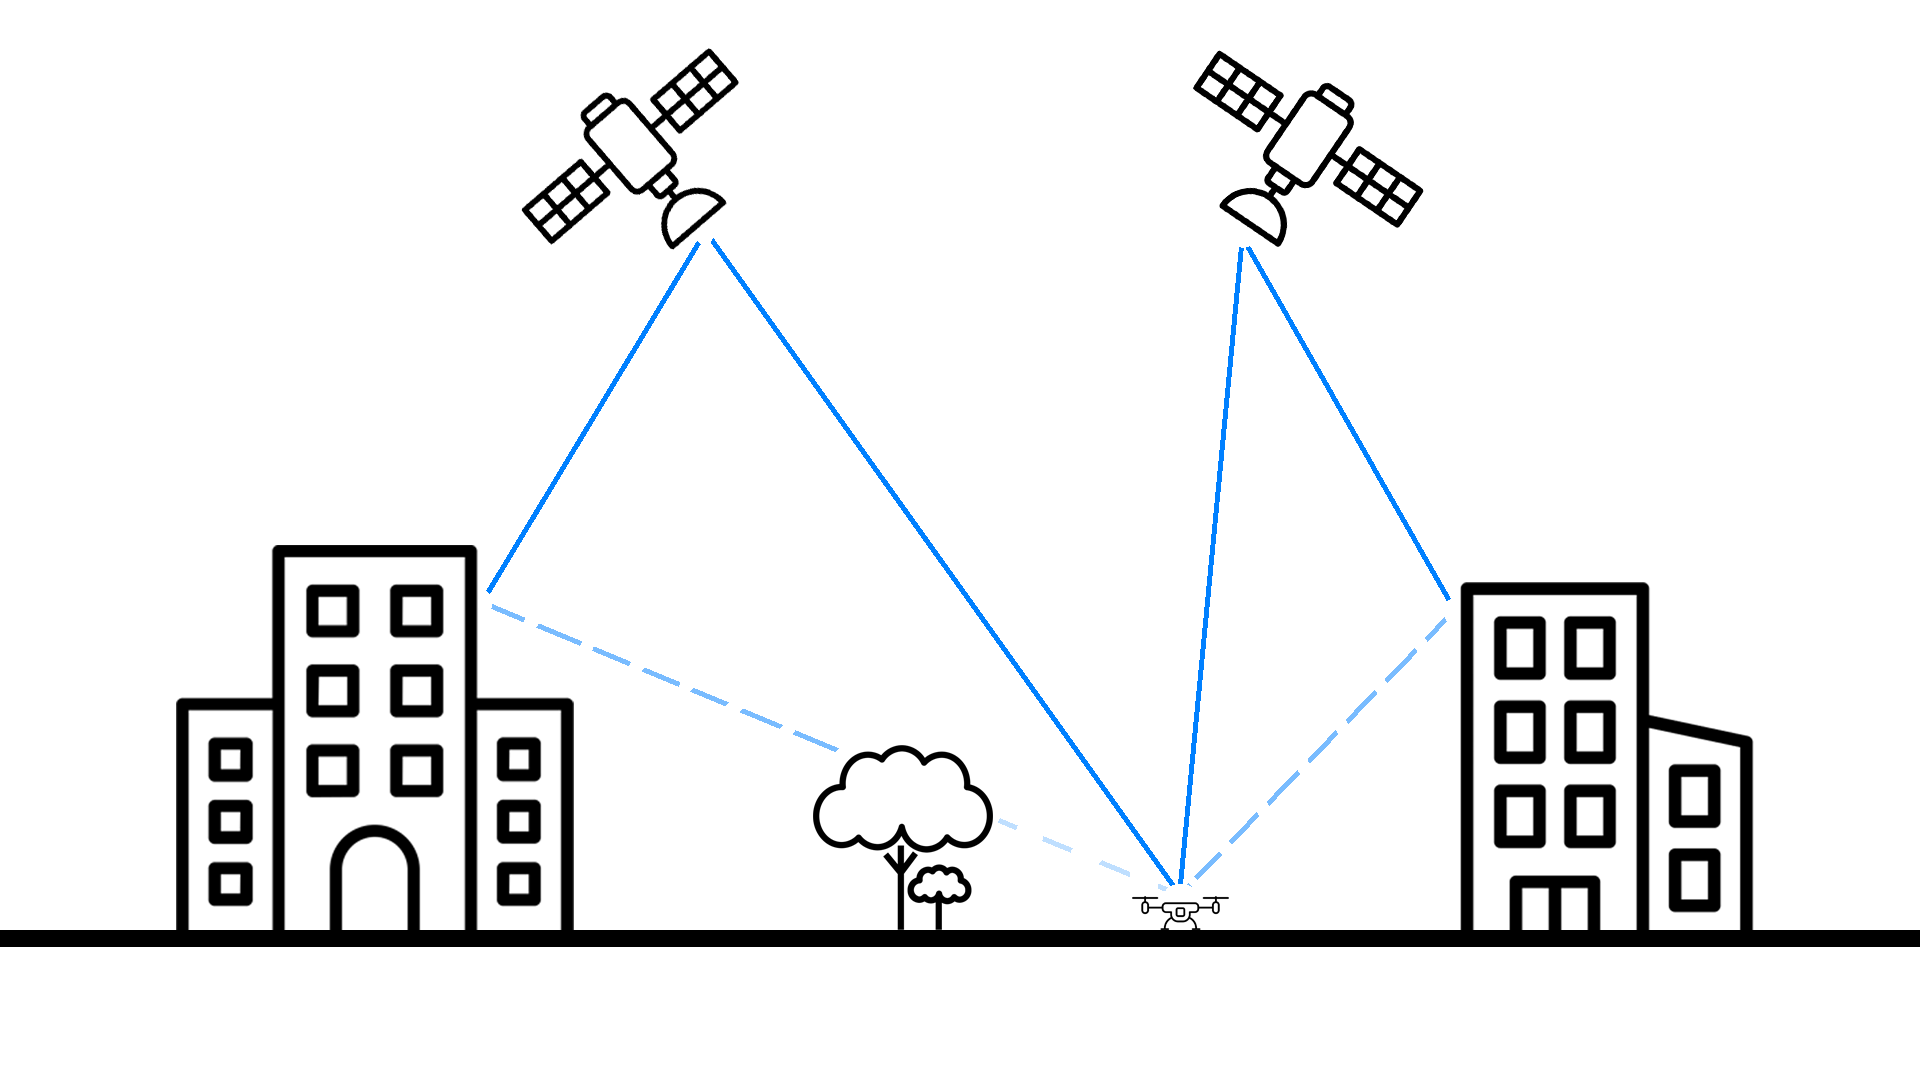
\includegraphics[width=1.0\textwidth]{Chapters/Figures/multipath.png}
	\caption{GNSS satellite signal multipath propagation.}
	\label{fig:multipath}
\end{figure}

% % example of multipath propagation:--------------------------------------
% As an example of the effects of mulipath propagation:
% If either the transmitter or the receiver, or both, are inside man-made structures, then additional propagation losses typically occur. These losses should be added (in decibels) to the propagation losses computed using the models described previously.
% Building penetration losses vary considerably with building construction, materials, structure, and the location of the receiver or transmitter within the building. The presence or absence of windows, and even the difference between metal window frames and wooden window frames, can make a significant difference in the propagation loss into a room. Besides propagation loss, signals received within a building often experience significant multipath.
% Building penetration losses are discussed extensively [41]. The following discussion is based on [40]. The excess loss in decibels due to building penetration is typically modeled, for signals arriving from above the building, as

% \begin{equation}
%     L=L_{roof}+n_{floor}\,L_{floor}\,,\medskip
% \end{equation}
% where
% - Lroof is the roof penetration loss, which can range from 1 dB to 30 dB at L-band;
% - nfloor is the number of floors penetrated;
% - Lfloor is the loss per floor, which can range from 1 dB to 10 dB at L-band. For building penetration through walls, the excess loss in decibels is similarly typically modeled as

% \begin{equation}
%     L=L_{ext}+n_{int}\,L_{int}\,,\medskip
% \end{equation}
% where
% - Lext is the exterior wall penetration loss, which can range from 1 dB to 30 dB at L-band;
% - nint is the number of interior walls penetrated;
% - Lint is the loss per interior wall, which can range from 1 dB to 10 dB at L-band.

% Table 9.13 lists representative losses for different building materials, drawing from an extensive set of measurements reported in [42].

% %meter tabela 9.13

% %----------------------------------------------------------------------

Regarding the reception of signals, it is intuitive that the more satellites that participate in the solution, the more accurate it will be, hence why the positioning is not restricted to just four satellites (as mentioned in Section~\ref{sec:II_gnss}) -- however, a direct line of sight is always required between any GNSS receiver that wants an accurate position and the (at least four) satellites. Being able to decode the satellites' signals due to their pseudo-random nature, the receivers are able to determine propagation times, and thus are also able to apply the methodology based on equation (\ref{eq:2_1}) to calculate ranges to the respective satellites.

% Receivers vary in terms of which constellation or constellations they track, and how many satellites they track simultaneously. For each satellite being tracked, the receiver determines the propagation time. It can do this because of the pseudorandom nature of the signals.

% Since the receiver knows the pseudorandom code for each satellite, it can determine the time it received the code from a particular satellite. In this way, it can determine the time of propagation.

% fim da parte de propagação.

% Important requirement: the requirement of CDMA to operate in a high bandwidth, therefore truly benefiting from this L-band.

% It was also specially selected to work on due to the fact that it

% C/A P-code~\cite{ca_p_code_1991}

It is also worth stating that the navigation message transmitted has a low bit rate, being that one of the reasons why these signals should be transmitted in high frequencies. Table~\ref{tab:GNSS_freqs} and Figure~\ref{fig:global_frequencies} show the frequencies that yield the best transmission results by each GNSS constellation signals~\cite{novatel_gnss,kaplan_2017,groves_2008}.

% % NOTA FINAL SOBRE GNSS:
% As more GNSS constellations are designed and more satellites are added, we will be able to calculate position more accurately and in even more places, expanding the already wide coverage of the planet.

% %falar de cada frequência: ...
% L5:
% The United States has implemented a third civil
% GPS frequency (L5) at 1176.45 MHz. The modernized
% GPS satellites (Block II-F and later) are
% transmitting L5.
% the modernied benefits of the L5 signal include meeting
% the requirements for critical safety-of-life applications
% such as that needed for civil aviation
% and providing:
% - Improved ionospheric correction.
% - Signal redundancy.
% - Improved signal accuracy.
% - Improved interference rejection.

\section{Precision improvement}\label{sec:II_gnssAug}

Regarding precise navigation, the precision obtained solely by relying on GNSS is not good enough (as it only offers meter-level accuracy~\cite{novatel_gnss}) -- as shown in Table~\ref{tab:GNSS_sys_errors}. Taking the example of an autonomous drone used in missions such as the ones mentioned in the begginning of Section~\ref{sec:II_gnss}, the need for a higher degree of precision is definitely clear. To make this type of navigation possible, the top priority is to bring GNSS system errors down to a minimum.

% no final meter tabela: ATENÇÃO À POSIÇÃO DA TABELA!!
\begingroup
\begin{table}[h]
	\caption{GNSS signals and frequencies.}
	\label{tab:GNSS_freqs}
	\centering%@{}l@{}@{}c@{}@{}c@{}@{}c@{}@{}c@{}
    % \setlength{\tabcolsep}{10pt} % Default value: 6pt
    % \renewcommand{\arraystretch}{1.5} % Default value: 1
	\begin{tabular}{lcc}
        \toprule

        \textbf{System} & \textbf{Signal} & \textbf{Frequency (MHz)} \\

        \midrule

        \multirow{5}*{GPS}      & L1 C/A    & 1575.42 \\
        \multirow{5}*{}         & L1C       & 1575.42 \\
        \multirow{5}*{}         & L2C       & 1227.60 \\
        \multirow{5}*{}         & L2P       & 1227.60 \\
        \multirow{5}*{}         & L5        & 1176.45 \\

        \midrule

        \multirow{4}*{GLONASS}  & L1 C/A    & 1598.0625-1609.3125 \\
        \multirow{4}*{}         & L2C       & 1242.9375-1251.6875 \\
        \multirow{4}*{}         & L2P       & 1242.9375-1251.6875 \\
        \multirow{4}*{}         & L3 OC     & 1202.025            \\

        \midrule

        \multirow{5}*{Galileo}  & E1        & 1575.42  \\
        \multirow{5}*{}         & E5a       & 1575.42  \\
        \multirow{5}*{}         & E5b       & 1207.14  \\
        \multirow{5}*{}         & E5 AltBOC & 1191.795 \\
        \multirow{5}*{}         & E6        & 1278.75  \\

        \midrule

        \multirow{6}*{BeiDou}   & B1l       & 1561.098 \\
        \multirow{6}*{}         & B2l       & 1207.14  \\
        \multirow{6}*{}         & B3l       & 1268.52  \\
        \multirow{6}*{}         & B1C       & 1575.42  \\
        \multirow{6}*{}         & B2a       & 1176.45  \\
        \multirow{6}*{}         & B2b       & 1207.14  \\

        \midrule

        NavIC     & L5        & 1176.45 \\

        \midrule

        \multirow{6}*{QZSS}     & L1C/A     & 1575.42 \\
        \multirow{6}*{}         & L1C       & 1575.42 \\
        \multirow{6}*{}         & L1S       & 1575.42 \\
        \multirow{6}*{}         & L2C       & 1227.6  \\
        \multirow{6}*{}         & L5        & 1176.45 \\
        \multirow{6}*{}         & L6        & 1278.75 \\

        \midrule

        \multirow{2}*{SBAS}     & L1        & 1575.42 \\
        \multirow{2}*{}         & L5        & 1176.45 \\

        \bottomrule
    \end{tabular}
\end{table}
\endgroup

At this point it is clear that the focal point behind GNSS positioning is related to equation (\ref{eq:2_1}), which means that any error connected to distance, velocity or time will affect the transmitted signal's quality, and thus, mitigation of these problems will yield better results.
The way to do so is through techniques relying on the augmentation of GNSS positioning capabilities~\cite{novatel_gnss,kaplan_2017}, which describes an ingenious way of improving the four performance parameters described earlier (accuracy, availability, continuity and integrity).
These techniques range from least to most effective, and can rely on:

\begin{itemize}
    \item Average calculation of recurring measurements at the same location;
    \item Prediction of correction values through modeling of the event causing the error;
    \item Differential Corrections (DGNSS).
\end{itemize}
DGNSS solutions represent the highest efficiency attainable. % citation needed

%meter imagem das frequencias de todas constelações no mesmo referencial: figura 36 novatel_gnss
% meter imagem svg do planeta com todas as GNSS?
\begin{figure}[ht]
	\centering
	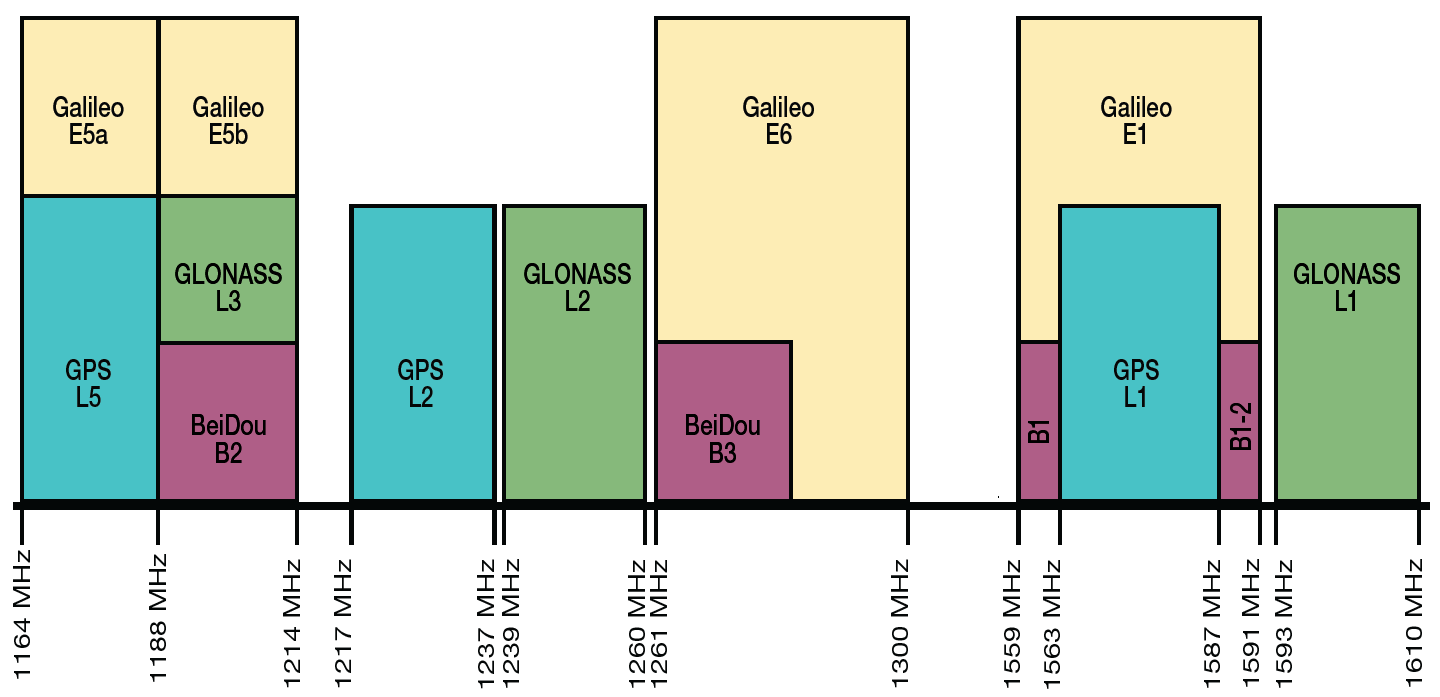
\includegraphics[width=1.0\textwidth]{Chapters/Figures/global_frequencies.png}
	\caption{Main frequencies used by all GNSS services (adapted from~\cite{novatel_gnss}).}
	\label{fig:global_frequencies}
\end{figure}

%For the purpose of this dissertation, the focus of error correction through GNSS augmentation will be set on differential corrections (more precisely, Differential GNSS, or DGNSS), as this is method relates directly with the beRTK\textsuperscript{\textregistered} base station.

% Breaking augmentation systems in a twofold way, accuracy and integrity ssuring further development of accuracy from GNSS augmentation

% % wiki:
% Based on its main feature, GNSS augmentation systems can be classified as those providing integrity information to the primary GNSS satellites constellation(s) and those improving the accuracy of the user solution with respect to the only use of the primary GNSS constellation(s).

% A further classification may be done according to an additional relevant feature, which for the former relates on whether the augmentation information comes from satellites (satellite-based augmentation system) or from ground (ground-based augmentation system) and for the latter on whether the accuracy improvements use a dense network of reference stations (Differential GNSS, Real Time Kinematics - RTK - or Wide Area RTK (WARTK)) or just a few stations (Precise Point Positioning - PPP) for the computation of the augmentation information.

% meter imagem: wiki Accuracy Performances for GNSS and GNSS Augmentation Techniques - METER (adapted from) !!!!!!!!!!!!!
% \begin{figure}[ht]
% 	\centering
% 	
\includegraphics[width=1.0\textwidth]{Chapters/Figures/demo.png}
% 	\caption{Accuracy Performances for GNSS and GNSS Augmentation Techniques.}
% 	\label{fig:accuracy_perfromances}
% \end{figure}

% --------------- PARTE A VERDE: DONE
The conventional code-based method stated in Section~\ref{sec:II_gnss_comm} is not capable of providing low-order levels of precision, so another method known as ``carrier-based'' was developed.
This type of method means that the measurement of the carrier wave's phase corresponds to a measurement of the distance (also known as range) between the satellite and the receiver, expressed in number of cycles of the carrier frequency~\cite{inside_GNSS} (Figure~\ref{fig:dgnss_corrections}), which results in more accurate output results, ideal for UAV missions.
Among the best-known techniques that adopt this method capable of calculating highly accurate solutions (i.e. orders of magnitude more accurate than those obtained through code-based GNSS) is Real-Time Kinematic (RTK) positioning\footnote{Real-Time Kinematic (RTK) positioning will be covered in more detail in Section~\ref{sec:II_gnssAug_rtk}.}, which is the main focus of the beRTK\textsuperscript{\textregistered} Base Station.
%meter imagem figura 40 base station a fazer correçoes:
\begin{figure}[h]
	\centering
	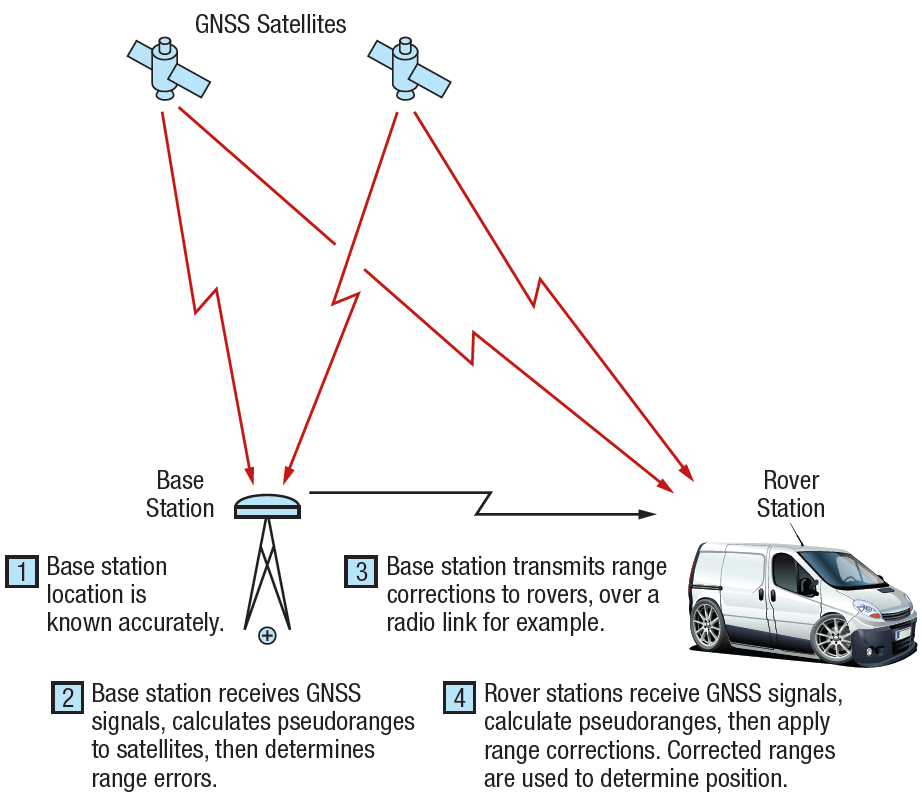
\includegraphics[width=1.0\textwidth]{Chapters/Figures/dgnss_corrections.png}
	\caption{Differential GNSS workings (adapted from~\cite{novatel_gnss}).}
	\label{fig:dgnss_corrections}
\end{figure}

Taking into account the possible signal ambiguities that may arise when using a carrier-based technique, the accuracy of the solution can only be maximized after they are resolved. This is possible through phase modulation of the carrier waves using a PRN code which, as mentioned, is capable of differentiating satellite signals, as well as making timing corrections in order to perform range calculations.
% ------------------ fim da PARTE VERDE.

\subsection{Differential GNSS}\label{sec:II_gnssAug_dgnss}

% --------------- PARTE VERMELHA: DONE
Looking again at Figure~\ref{fig:dgnss_corrections}, a depiction of one of the most important devices for augmented GNSS services can clearly be seen: the base station. This element is crucial to the workings of the technique able to describe the operation of RTK, known as Differential GNSS, or DGNSS. This carrier-based method consists on the use of a base station (i.e. a fixed GNSS receiver) that sits in a static and known position (obtained in a highly accurate way through conventional surveying techniques). Due to the nature of the internal GNSS receiver, the ranges to each GNSS satellite in line of sight are effectively determined using a code-based technique (conventional GNSS positioning), and the location of each of these satellites is also calculated taking into account precisely known orbit ephemerides as well as the current time of the internal atomic clock of each satellite.
When comparing the measured position with the calculated one (from the ranges to each satellite -- also calculated), it can be clearly assumed that the differences between both positions will be ephemeris-related, as well as due to the differences between clocks
%relative clock offsets (?)
-- bearing in mind that, unlike a GNSS satellite, a base station does not have an atomic clock. However, delays related to the passage of the signal through the atmosphere are the most recurring and common errors.
Subsequently, in order for the corrections to be incorporated in the calculated solutions, the base station performs the task of sending the detected range errors to other receivers that also obtain their position through GNSS positioning (rovers, e.g. a UAV). This correlation allows such errors to be calibrated out.
For this, it is necessary to establish a link for the supply of data between the base station and the rover, keeping in mind the fast transmission and reception of corrections happening in real-time. Connections like these can be made through radio frequency\footnote{The LoRa protocol is good example for this.} -- by using a frequency interval with values ranging from under 300 kHz (low frequencies, or LF) to around 1-2 GHz (corresponding to the L-band (first mentioned in Section~\ref{sec:II_gnss_comm})) and above -- or the internet.

In case the need arises for a quick calculation of corrections, i.e. in real-time, both devices will need to have in their line of sight at least four GNSS satellites -- three for the determination of the position according to $x$, $y$ and $z$ and an extra one to correct for clock time differences between satellites and receivers, commonly called ``time offset''. Thus, it is concluded that, in order to obtain a high-precision position for the rover, a high-precision position must first be determined at the base station, considering the dependence between the two. If it is assumed that, for the missions performed, the rover does not move too far from the base station, the real-time accuracy of the measurements will be high, taking into account that the signals received by each of the devices will pass through, sensibly, the same atmosphere conditions. In this way, the greater the distance possible to maintain between devices, the better.

% If one wishes to put aside the real-time factor of the job, there are other techniques capable of providing precise positioning -- in some cases, the precision values may even be higher than those obtained from RTK -- by using two GNSS receivers trusted with the task of logging positioning data to a storage device. Later, the gathered data can be processed however it's intended to. Section~\ref{sec:II_gnssAug_ppk} describes an example of such method, known as \gls{PPK}~\cite{novatel_gnss,kaplan_2017,groves_2008}.
% % ------------------ fim da PARTE VERMELHA.

% \subsection{Satellite-based Augmentation System (SBAS)}\label{sec:II_gnssAug_sbas}

% % --------------- PARTE A LARANJA:
% Table~\ref{tab:GNSS_freqs} introduced various frequency values for different GNSS constellations, with all of them having already been addressed, except one: indicated as \gls{SBAS}.

% SBAS's design purpose has in mind situations where the usage and financial value of the DGNSS can be circumvented, mainly due to the possibility of spreading the base stations over a very wide area of work. It should be noted that the focus of this system has a lot to do with large-scale work areas, which are where SBAS proliferates.

% Making use of geosynchronous satellites, i.e. satellites that orbit the Earth with a period equivalent to its rotation, these systems work as auxiliaries of the currently existing GNSS networks, as they are also able to improve signal parameters such as:
% \begin{itemize}
%     \item Accuracy: Possible to be improved by propagating wide area corrections for all detected GNSS range errors;
%     \item Availability: In a straightforward way, signal availability is possible to improve through the transmission of range signals from each SBAS satellites;
%     \item Integrity: Ensured by the SBAS network via rapid detection of satellite signal errors and subsequent sending of non-tracking alerts to the receivers.
% \end{itemize}

% %meter imagem dos SBAS systems: DONE
% \begin{figure}[ht]
% 	\centering
% 	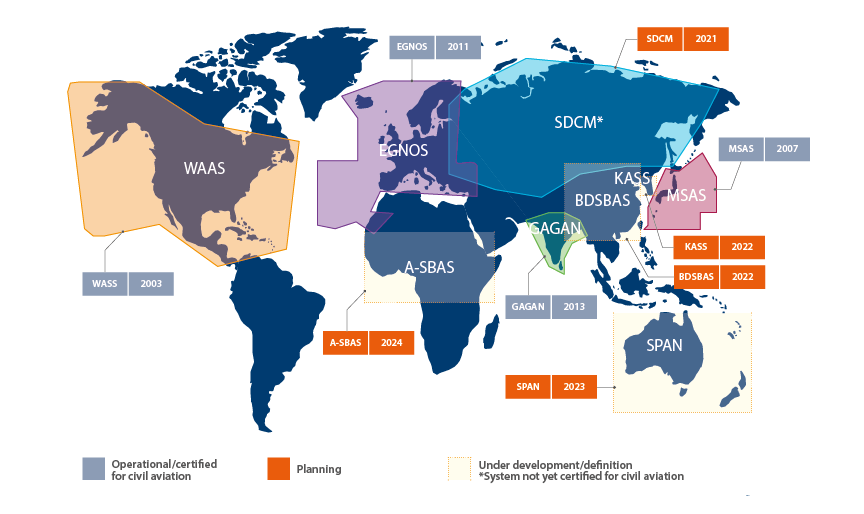
\includegraphics[width=1.0\textwidth]{Chapters/Figures/SBAS.png}
% 	\caption{SBAS systems (currently in operation/development; adapted from~\cite{sbas_euspa_2021}).}
% 	\label{fig:SBAS_systems}
% \end{figure}

% Currently, there are several SBAS services implemented that provide extra positioning precision. Figure~\ref{fig:SBAS_systems} shows the already existing SBAS, as well as the ones in current development, which are:
% \begin{itemize}
%     \item Wide Area Augmentation System (WAAS): Developed by the U.S. Federal Aviation Administration (FAA);
%     \item System for Differential Corrections and Monitoring (SDCM): Currently in development by the Russian Federation;
%     \item European Geostationary Navigation Overlay Service (EGNOS): Developed by the European Space Agency (ESA), in cooperation with the European Commission (EC) and EUROCONTROL (European Organization for the Safety of Air Navigation). Provides coverage to the majority of the European Union (EU);
%     \item BeiDou SBAS (BDSBAS): Currently in development by the People's Republic of China;
%     \item GPS-aided GEO-Augmented Navigation (GAGAN): Developed by the Indian government;
%     \item Michibiki Satellite Augmentation System (MSAS): Developed by the Japanese government;
%     \item Korea Augmentation Satellite System (KASS): Currently in development by the Korea Aerospace Research Institute (KARI);
%     \item Southern Positioning Augmentation Network (SPAN): Currently in development by Australia and New Zealand;
%     \item ASECNA's SBAS for Africa and Indian Ocean (A-SBAS): Currently in development by the Agency for Air Navigation Safety in Africa and Madagascar (ASECNA), Nigerian Communications Satellite Ltd. (NIGCOMSAT) and Thales Alenia Space~\cite{a_sbas_2021}.
% \end{itemize}
% It should also be noted that the services provided by all these systems are compatible and interoperable, which means all the systems themselves also are~\cite{novatel_gnss,kaplan_2017,sbas_euspa_2021}.
% ------------------ fim da PARTE LARANJA.

% Ground Based Augmentation System: % meter wiki disto:
% Ground-Based Augmentation System (GBAS) aim at enhancing GNSS service levels for aviation during approach, landing and departure phases, as well as for surface operations. They have a local coverage (e.g. the surroundings of an airport) with the primary objective of meeting aviation requirements for the aforementioned operations and phases, in terms of accuracy, integrity and safety. Actually, whereas the main goal of GBAS is to provide integrity assurance, it also increases the accuracy with position errors below 1 m (1 sigma).

% The ground infrastructure includes two or more GNSS receivers which collect pseudoranges for all the primary GNSS satellites in view and computes and broadcasts differential corrections and integrity-related information for them based on its own surveyed position. These differential corrections are transmitted from the ground system via a Very High Frequency (VHF) Data Broadcast (VDB). The broadcast information includes pseudorange corrections, integrity parameters and various locally relevant data such as Final Approach Segment (FAS) data, referenced to the World Geodetic System (WGS-84). Any aircraft (within the area of coverage of the ground station) may use those corrections to compute their own measurements to compute a (differentially corrected) position, which at the same time is used to generate navigation guidance signals.

% GBAS and SBAS are both GNSS safety critical systems for civil aviation which share similar principles. The main difference comes from the fact that GBAS provides local corrections to the satellite pseudoranges using just ground infrastructure in the vicinity of the served airport, whilst SBAS broadcasts corrections to the different components of the pseudorange error valid for an area as big as a continent; the price to pay is that the SBAS infrastructure needs tens of sensor distributed in the augmented area and two or more GEO satellites to broadcast the information.


% %wiki: ..................
% A Satellite Based Augmentation System (SBAS) is a civil aviation safety-critical system that supports wide-area or regional augmentation - even continental scale - through the use of geostationary (GEO) satellites which broadcast the augmentation information[1][2]. A SBAS augments primary GNSS constellation(s) by providing GEO ranging, integrity and correction information. While the main goal of SBAS is to provide integrity assurance, it also increases the accuracy with position errors below 1 metre (1 sigma).

% The ground infrastructure includes the accurately-surveyed sensor stations which receive the data from the primary GNSS satellites and a Central Processing Facility (CPF) which computes integrity, corrections and GEO ranging data forming the SBAS signal-in-space (SIS). The SBAS GEO satellites relay the SIS to the SBAS users which determine their position and time information. For this, they use measurements and satellite positions both from the primary GNSS constellation(s) and the SBAS GEO satellites and apply the SBAS correction data and its integrity.

% The augmentation information provided by SBAS covers corrections and integrity for satellite position errors, satellite clock - time - errors and errors induced by the estimation of the delay of the signal while crossing the ionosphere. For the errors induced by the estimation of the delay caused by the troposphere and its integrity, the user applies a tropospheric delay model.

% SBAS systems, such as EGNOS or WAAS, are usable for the safety-critical task of guiding aircraft -vertically as well as horizontally- during different operations, including landing approaches (approach with vertical guidance, APV).
% %............................

% Used to provide integrity assurance;
% Used to increase accuracy and to reduce position errors to less than 1 meter.
% "Augmentation of a global navigation satellite system (GNSS) is a method of improving the navigation system's attributes, such as accuracy, reliability, and availability, through the integration of external information into the calculation process."

\subsection{Real-Time Kinematic (RTK)}\label{sec:II_gnssAug_rtk}

%parte AMARELA: --------------------
As mentioned earlier, carrier-based methods are the go-to when dealing with navigation in a real-time scenario, which perfectly describes Real-Time Kinematic positioning, a method that is precisely one of the main topics of this Dissertation.

RTK fits, as indicated, in situations where high precision is indispensable for the performance of a certain task (e.g. use of a UAV to distribute pesticides in an agricultural field); as such, the accuracy levels obtained should be of the smallest order possible -- recalling Table~\ref{tab:GNSS_sys_errors}, which, from an RTK standpoint, would be unacceptable.

%meter imagem da Figura 42 - base station + rover RTK
\begin{figure}[ht]
	\centering
	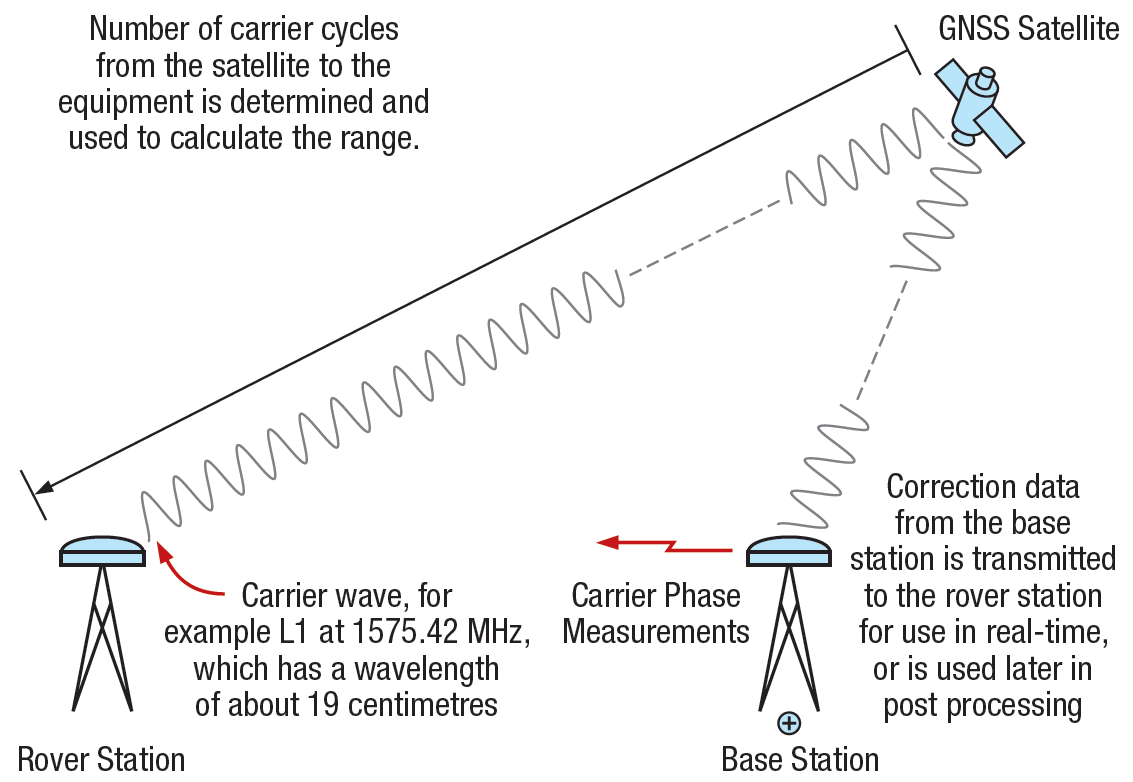
\includegraphics[width=1.0\textwidth]{Chapters/Figures/rtk_workings.png}
	\caption{RTK positioning (adapted from~\cite{novatel_gnss}).}
	\label{fig:rtk_workings}
\end{figure}

Observing Figure~\ref{fig:rtk_workings}, the base station-rover pair can be seen again, so it is possible to draw an analogy from Figure~\ref{fig:dgnss_corrections}. The basic operation behind this precise positioning method consists, essentially, in the process characterised by the detection and correction of positioning errors through the determination of ranges to GNSS satellites -- again based on equation (\ref{eq:2_1}). Conceptually, the calculation of these ranges is performed as explained in Section~\ref{sec:II_gnssAug}, with regard to the carrier-based methodology: by calculating the number of cycles of the carrier wave between the satellite and the receiver installed on the rover ($n$) and multiplying it by its own wavelength ($\lambda$), where

\begin{equation}\label{eq:2_4}
    \lambda = \frac{v}{f}\medskip
\end{equation}
In this case, $v$ and $f$ are the propagation velocity and frequency of the carrier wave, respectively.

However, the calculations performed will inevitably continue to carry range errors related to the already known effects intrinsic to satellite clocks and the Earth's atmosphere. It is precisely at this stage that the rover's positioning corrections by the base station come in, corrections that are then transmitted through, typically, a radiofrequency link.

As explained in~\ref{sec:II_gnssAug}, the use of a technique based on carrier waves often leads to ambiguity problems, so their resolution must be prioritized, so that it is possible to determine the number of complete cycles ($n$), properly taking advantage of the calculated corrections -- this can be done with the help of PRN codes, which, in high-precision GNSS receivers, happens almost instantly.

Thus, it is known that the ability to determine the exact position in RTK positioning depends on the correction of errors derived from the sources already stated, which confirms the use of the term ``differential'', as used in the DGNSS technique, since the determination of the rover's position in both methods depends on a base station. However, the crucial difference between these methods lies in the fact that the latter makes use of a code-based methodology, which, as it is known, leads to results with lower precision than those obtained using a carrier-based methodology. Note also from Figure~\ref{fig:rtk_workings} that there is yet another factor to be considered for the accuracy of measurements, which is the distance from the base station itself to the rover, known as ``baseline''.
As it can be intuitively deduced, the variation of this distance also causes a variation in the accuracy of the determined location. When compared to RTK positioning, the DGNSS positioning technique allows greater baselines, which is due to the use of code-based methodology. However, the trade-off occurs, as stated, at lower precision values.
% Baseline in RTK mode and Baseline in PPK mode -- for different projects, a different distance from the rover to the base might be needed. Working near a city is more likely to have base station stations nearby. However, when working in rural areas, base stations are likely to be further away.
% Multi-band receivers can work at a longer baseline due to the use of multiple satellite constellations -- as these help in the correction of the readings taken by the base, as mentioned before (earlier?). beRTK\textsuperscript{\textregistered} can operate with the baseline up to 2.5 km.
% fazer uma imagem parecida a esta:
% meter imagem da baseline Emlid

Also not represented in Figure~\ref{fig:rtk_workings} is a factor that impacts accuracy: the positioning of the base station. This parameter should not be neglected in any way, since, when connections are established through radiofrequency with a rover, the propagation of correction information will be done, as the term implies, through radio waves; due to their nature, these waves may suffer the same problems already observed in the propagation of waves from GNSS satellites -- such as interference and multipath --, so the location selection is important to minimize all negative effects. Another way to do this could also be to improve the quality of the rover's antennas~\cite{novatel_gnss,ayers_geosystems_2011,8093778,9292033}.
% ------------------ fim da PARTE AMARELA.

% %MUDAR, ESTÁ COPIADO!
% So, the difference between RTK and DGPS is that DGPS is the traditional differential GPS.
% RTK is a specific type of DGPS.
% but it uses a newer technology than the traditional DGPS.
% RTK stands for real-time kinematic and commonly uses the RTCM protocol.
% The traditional DGPS uses an older antiquated protocol while RTK uses a newer algorithm, and the protocol is based on RTCM3. data flow rate is much higher in RTK.
% %____________

% - Used to improve the accuracy of standalone GNSS receivers. Traditional GNSS receivers can only determine the position with na accuracy of about 2-4 meters (?). RTK provides centimeter accuracy.
% - GNSS receiver measure how long it takes for a signal to travel from a satellite to the receiver. Due to the presence of atmosphere between the satellite and the receiver, the transmitted signals are slowed down and are introduced to perturbations. With this in mind, one can immediately assume that transmission times will differ according to the weather at the time of the event. That is the reason why a standalone receiver has a hard time determining its position accurately. RTK is a Technology that solves this issue.
% - 2 receivers are used in RTK. One of them is stationary, the other is a moving rover.
% - Real Time Kinematic (RTK) is a GPS correction technology technique that provides real-time corrections to location data as the drone is surveying and capturing images from a site.


\subsection{Networked RTK}\label{sec:II_networkedRTK}

Obtaining position corrections with RTK can also be done in a way that does not require the aid of a base station set up by the end-user -- through a process known as Networked RTK.
It is a technique that relies on the use of stations permanently fixed at known and spaced positions -- which are, essentially, base stations -- to obtain positioning corrections over the internet. Thus, this process can be seen for what it literally is: a way to obtain positioning corrections through a network of virtual base stations, which immediately leads to a general reduction in the quantity of RTK base stations necessary, as well as to the conclusion that long baselines cease to be a problem.

As stated in Section~\ref{sec:II_gnss_comm}, if a receiver relies solely on satellite signals for positioning, the rate at which information will be received will be rather low. Relying on internet connection to get position corrections is a great way to bypass such problem. The use of a \gls{CORS} network is an example of networked RTK. Its operation is based on the use of stations that are permanently installed in previously known and properly interspaced locations, making regular observations of the GNSS satellites correcting any errors based on such~\cite{novatel_gnss}.
Most countries have systems of this kind, which are openly accessible to the public. In addition to helping with positioning corrections, CORS stations can also transmit (through knowledge of their position) information about changes in the Earth's surface, thus helping to detect any tectonic movements -- which, in consequence, assists in measuring earthquakes and volcanic eruptions. An example of such is the Portuguese CORS network (ReNEP\footnote{Accessible through \url{https://renep.dgterritorio.gov.pt}.}); consisting of 47 permanent GNSS stations throughout the country, this system provides not only navigation information but also information about the tectonic plate on which a particular station is located~\cite{ReNEP_ppt_2018}.

\subsubsection{NTRIP}\label{sec:II_networkedRTK_ntrip}

%daniel:
The next step when dealing with the virtual base stations is for the rover to effectively fetch their positioning data from the internet so that the corrections can be made. For that, a protocol known as NTRIP (Networked Transport of RTCM via Internet Protocol) can be used (Figure~\ref{fig:ntrip_network}). This protocol is used to effectively make the use of a second GNSS receiver obsolete by establishing a virtual link between the rover and base stations, through the internet. The latter then detects and corrects the errors, subsequently forwarding the treated data to the rover. The connection can be made through an already familiar radiofrequency link -- this time, to the internet itself -- or another chosen wireless medium.

Figure~\ref{fig:ntrip_network} also represents the three main sectors that constitute an NTRIP-based environment:

\begin{itemize}
    \item Base: Usually a CORS reference/base station -- assured to be in continuous operation; used to detect errors and calculate precise solutions;
    \item NTRIP caster: An HTTP internet service that forwards the connection data through the internet;
    \item Rover: The client's rover receiver used in real-time precise positioning solutions.
\end{itemize}
% \includegraphics[width=1.0\textwidth]{Chapters/Figure
%meter imagem NTRIP da Emlid:
\begin{figure}[ht]
	\centering
	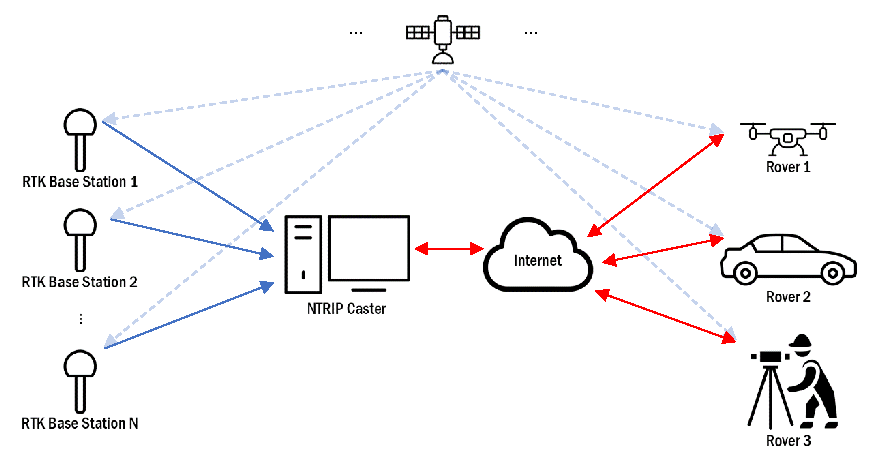
\includegraphics[width=1.0\textwidth]{Chapters/Figures/ntrip_network.pdf}
	\caption{Network RTK positioning using NTRIP.}
	\label{fig:ntrip_network}
\end{figure}

The standards used in RTK systems are able to follow more than one specific format (which are the same used in DGNSS systems); the most widely used are the \gls{CMR} and \gls{RTCM} (or RTCM SC-104) standards. These two branch out into the following formats acceptable by NTRIP networks: CMR, CMR+, RTCM 2.x and RTCM 3.x. Only available for GPS services, the first three formats became less used after the introduction of the third version of the RTCM standard in 2003, which restructured the previous formats to the parameters presented in Table~\ref{tab:rtcm_messages}.
%table:
\begingroup
\begin{table}[h]
	\captionsetup{justification=centering}
    \caption{RTCM version 3 structural frame (adapted from~\cite{rtcm_china}).}
	\label{tab:rtcm_messages}
	\centering%@{}l@{}@{}c@{}@{}c@{}@{}c@{}@{}c@{}
    % \setlength{\tabcolsep}{10pt} % Default value: 6pt
    % \renewcommand{\arraystretch}{1.5} % Default value: 1
	\begin{tabular}{ccccc}
        \toprule
        \multirow{2}*{\textbf{Preamble}} & \multirow{2}*{\textbf{Reserved}} & \textbf{Message} & \textbf{Variable Length}     & \multirow{2}*{\textbf{CRC}} \\
                                         &                                  & \textbf{Length}  & \textbf{Data Message}        &                             \\

        \midrule
        \multirow{2}*{8 bits} & \multirow{2}*{6 bits} & \multirow{2}*{10 bits} & Variable length,         & \multirow{2}*{24 bits} \\
                              &                       &                        & integer number of bytes &                        \\
        \bottomrule
    \end{tabular}
\end{table}
\endgroup

\begingroup
\begin{table}[h]
	\captionsetup{justification=centering}
    \caption{Most common RTCM version 3 message codes used in RTK applications (adapted from~\cite{rtcm_cheat_sheet}).}
	\label{tab:rtcm_codes}
	\centering%@{}l@{}@{}c@{}@{}c@{}@{}c@{}@{}c@{}
    % \setlength{\tabcolsep}{10pt} % Default value: 6pt
    % \renewcommand{\arraystretch}{1.5} % Default value: 1
	\begin{tabular}{ll}
        \toprule
        \textbf{Code} & \textbf{Message} \\
        \midrule
        \multirow{2}*{1004} & Extended L1 and L2 GPS RTK observables for GPS RTK use; the \\
                            & main message \\
        \midrule
        1005 & Stationary RTK Reference Station ARP \\
        \midrule
        1006 & Stationary RTK Reference Station ARP plus the antenna height \\
        \midrule
        1007 & Antenna Descriptor \\
        \midrule
        \multirow{2}*{1012} & Extended L1 and L2 GLONASS RTK observables; the other main \\
                            & message \\
        \midrule
        1013 & System Parameters, time offsets, lists of messages sent \\
        \midrule
        1017 & GPS Combined Geometric and Ionospheric Correction Differences \\
        \midrule
        1019 & GPS Broadcast Ephemeris (orbits) \\
        \midrule
        1020 & GLONASS Broadcast Ephemeris (orbits) \\
        \midrule
        1029 & Unicode Text String (used for human-readable text) \\
        \midrule
        1033 & Receiver and Antenna Descriptors \\
        \midrule
        1045 & Galileo Broadcast Ephemeris \\
        \bottomrule
    \end{tabular}
\end{table}
\endgroup

In order for the messages to be understood by receivers in a more efficient way, a code specific to each message is defined. Table~\ref{tab:rtcm_codes} shows an adaptation of the most common codes used in RTK positioning~\cite{ntrip_agleader,rtcm_tuga,rtcm_china}.

With all this in mind, it is also possible to understand that, due to the connection of a GNSS receiver to an NTRIP network, it will be able to start by collecting a more precise location faster. This is commonly known as having ``faster convergence'', which is a very important variable when describing a certain device capable of precise positioning.

% https://www.youtube.com/watch?v=uytd48Vb-fs&ab_channel=RamiTamimi
% "NTRIP (Network Transport of RTCM via Internet Protocol) and CORS (Continuously Operating Reference Station) are forms of RTK differential correction that are done using a cellular modem and base station network."
% "how to obtain high accuracy positioning utilising just one GNSS recevier?
% As described in Section~ (\textbf{ref}) , it is possible obtain high accuracy positioning by setting up two GNSS receivers, which will act as a base station and a rover. Therefore, this method requires double the cost of the method presented in this Section~. There is a way to use only one GNSS receiver and have RTK-enabled positioning, through the use of a CORS (Continuously Operating Reference System) network.% corte aqui
% These stations are permanentely set up on a single known location, and continue to observe satellites and perform corrections based on any errors that they observe. Most municipalities, states and countries own these systems and allow public access to anyone that sets up an account.

% next:
% Depending on the implementation, positioning data from the permanent stations is regularly communicated to a central processing station.
% On demand from RTK user terminals, which transmit their approximate location to the central station, the central station calculates and transmits correction information or corrected position to the RTK user terminal.
% The benefit of this approach is an overall reduction in the number of RTK base stations required. Depending on the implementation, data may be transmitted over cellular radio links or other wireless medium.


% If there are no NTRIP stations within a radius of (?) from the intended mission site, a base station will be needed in order to obtain the precise positioning through RTK, as described in~\ref{sec:II_gnssAug_rtk}.
% "it is very fast to obtain a fix. Rather than utilising our own base station for the corrections, the public NTRIP network is used, and the receiver (rover) will be connected to a base station in that network."
% Fazer uma imagem parecida a esta: % ver Word

% An internet based application that makes the RTCM Correction data from the CORS stations available to anyone with an internet connection and the appropriate log on credentials to the NTRIP server. Typically uses a mobile link to get to the internet and the NTRIP server. % https://www.teejet.com/CMSImages/TEEJET/documents/technical-updates/98-01410%20r0%20en%20tech%20update%20ntrip%20rx610.pdf

%se calhar nao sao precisas estas subsubsections! tirar!:

%references: \cite{,ntrip_agleader}

% \subsubsection{LoRa -- meter na footnote}\label{sec:II_gnssAug_rtk_LoRa}
% ``There are number of communication technologies available for interaction between IoT devices today, and the most popular ones are Wi-Fi and Bluetooth. But the problem with Wi-Fi and Bluetooth technology is high power consumption. They also have other limitations like limited range, limited access points etc. ESP8266 module is the most popular Wi-Fi module used in IoT devices, using which we have previously built lot of IoT projects.

% Cellular networks also have the same problems of high power consumption and both LAN and Cellular network are quite expensive to cover a wide area. The IoT industries introduced lots of technologies, but none of them was ideal for IoT devices, as they needed to transmit information to long distance without using much power, until the LoRa technology was introduced. LoRa Technology can perform very-long range transmission with low power consumption.

% LoRa (Long Range) is a wireless technology that offers long-range, low power, and secure data transmission for M2M (Machine to Machine) and IoT applications. LoRa is a spread spectrum modulation technology that is derived from chirp spread spectrum (CSS) technology. LoRa can be used to connect sensors, gateways, machines, devices, etc. wirelessly. In Europe region, it operates in the 868 MHz band.'' % https://iotdesignpro.com/projects/lora-communication-between-two-arduino-using-LoRa-Module-SX1278

% \subsection{Post-Processed Kinematic (PPK)}\label{sec:II_gnssAug_ppk}

% As mentioned in Section~\ref{sec:II_gnssAug_dgnss}, a technique that does not require real-time processing is Post-Processed Kinematic positioning. In this technique all known algorithms used are applied after completion of any given mission. That is, both the base station and the rover only need to collect and record positioning data on a storage device, so that, at a later stage, they are processed in the desired way, as often as needed. Thus, as the urgency factor imposed by a real-time application is removed from the equation, the results obtained through this technique will be more accurate than those obtained through RTK, allowing to work with larger baselines, which means the possibility of working in wider regions.
% Thus, PPK positioning is mostly used in UAV mapping applications~\cite{novatel_gnss}.

% \subsection{Precise Point Positioning (PPP)}\label{sec:II_gnssAug_ppp}

% %novatel:
% PPP is a positioning technique that removes or models GNSS system errors to provide a high level of position accuracy from a single receiver. A PPP  solution depends on GNSS satellite clock and orbit corrections, generated from a network of global reference stations. Once the corrections are calculated, they are delivered to the end user via satellite or over the Internet.
% These corrections are used by the receiver, resulting in decimetre-level or better positioning with no base station required. A typical PPP solution requires a period of time to converge to decimetre accuracy in order to resolve any local biases such as the atmospheric conditions, multipath environment and satellite geometry. The actual accuracy achieved and the convergence time required is dependent on the quality of the corrections and how they are applied in the receiver.
% Up to 3 centimetre accuracy is possible. Similar in structure to an SBAS system, a PPP system provides corrections to a receiver to increase position accuracy. However, PPP systems typically provide a greater level of accuracy and charge a fee to access the corrections.
% PPP systems also allow a single correction stream to be used worldwide, while SBAS systems are regional. A typical PPP system is shown in Figure 43.
% The main error sources for PPP are mitigated in following ways:
% - DUAL-FREQUENCY OPERATION: The firstorder ionospheric delay is proportional to the carrier wave frequency. Therefore, the first-order ionospheric delay can totally be eliminated by using the combinations of dual-frequency GNSS measurements.
% - EXTERNAL ERROR CORRECTION DATA: This includes satellite orbit and clock corrections. In the case of TerraStar service, the corrections generated are broadcast for end-users by Inmarsat telecommunication satellites.
% - MODELING: The tropospheric delay is corrected using the UNB model developed by the University of New Brunswick. However, the wet part of tropospheric delay is highly varying and it cannot be modeled with sufficient accuracy. Thus, residual tropospheric delay is estimated when estimating position and other unknowns. Modeling is also used in the PPP receiver to correct the solid earth tides effect.
% - PPP FILTER ALGORITHMS: An Extended Kalman Filter (EKF) is used for the PPP estimation. Position, receiver clock error, tropospheric delay and carrier-phase ambiguities are estimated EKF states. EKF minimizes noise in the system and enables estimating position with centimetrelevel accuracy. The estimates for the EKF states are improved with successive GNSS measurements, until they converge to stable and accurate values. The typical convergence time of PPP to under 10 cm horizontal error is between 20 and 40 minutes, but it depends on the number of satellites available, satellite geometry, quality of the correction products, receiver multipath environment and atmospheric conditions.
% There are several providers of PPP services, including, VERIPOS, TerraStar, OmniSTAR and StarFire. PPP service providers operate a network of ground reference stations to collect correction data for the different signals broadcast by each satellite. The corrections calculated from this data are broadcast from geostationary satellites to the receivers of subscribed users. More information about PPP is also available in the Advanced GNSS Positioning Solution article in the 2014 Velocity magazine.

% %daniel, mas nao foi o daniel:
% - A standalone receiver finds out its position relying on the data obtained from satellites only. Along with raw data from those satellites, the receiver gets navigation messages with satellite clock offset, ionospheric and tropospheric corrections (atmospheric-related disturbances), etc. Due to information about these offsets, the receiver may calculate its position with a few meters' accuracy. If there were (was) no navigation data, the accuracy would be much worse.
% - In RTK and PPK, these offsets might be eliminated since both (the) base station and the rover operate in quite similar conditions.
% - PPP allows the single receiver (rover) to achieve high-level accuracy without the use of corrections from the base station.
% - To calculate the coordinates, PPP uses the same data that is provided by the navigation message but much more accurate. Thereby, the single receiver (rover) might determine its position with a centimetre-level accuracy using only raw data and precise ephemerides and clock offsets provided by a PPP service.
% - The PPP technique is commonly used for determining the absolute base position for further RTK/PPK surveys.

% \section{Battery System}\label{sec:II_battery}
% % falar de todos os topicos que estejam no doc Word Battery

% The formula is (Wh)/(h) = (W). For example, if you have 100 Wh for a duration of 2 hours, then the wattage is (100)/(2) = (50) Watts.
% (Watthours is a measure of energy and watts is a unit of power. Power multiplied by time is enery).

% como cada uma das baterias atualmente em uso is rated for (as?) 7.4V, 1070 mAh, that corresponds to 7.918 Wh.

% % LiFePO$_4$ better than Li-ion batteries?
% ``The LiFePO$_4$ battery has the edge over lithium-ion, both in terms of cycle life (it lasts 4-5x longer), and safety. This is a key advantage because lithium ion batteries can overheat and even catch fire, while LiFePO4 does not''% citation needed

% \subsection{USB Type-C}\label{sec:II_usb_c}
% % ler wiki do USB-C e derivar os topicos daí
% % depois ir ao IEEEXplore procurar papers que dêem backup

% \subsubsection{Power Delivery}\label{sec:II_usb_c_PD}
% % PD is a protocol

\section{Current Solutions}\label{sec:II_curr_solutions}

This section aims to clarify the exposed concepts about the device representing the center of the project covered by this Dissertation: the RTK base station. For that, important parameters of some of the most relevant solutions currently available in the market are presented in Tables~\ref{tab:curr_sol_POSITIONING},~\ref{tab:curr_sol_ELECTRICAL},~\ref{tab:curr_sol_CONNECTIONS} and~\ref{tab:curr_sol_MECH}, which represent positioning, connectivity, electrical, and physical/mechanical characteristics, respectively.

\begingroup
\begin{table}[h]
    \centering
	\captionsetup{justification=centering}
    \caption{Some current base station solutions: positioning properties.}
    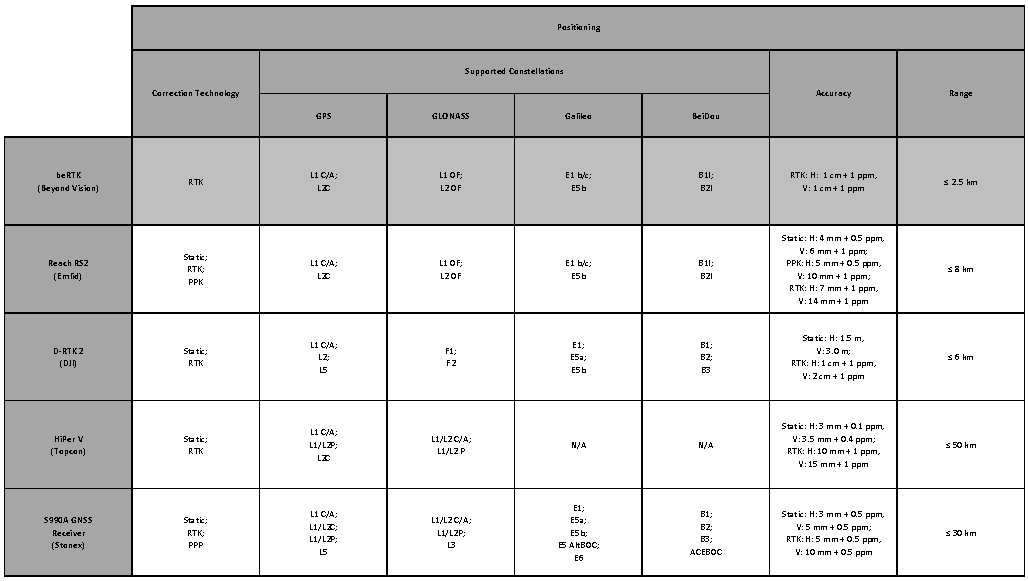
\includegraphics[width=1.0\textwidth]{Chapters/Figures/curr_solutions/POSITIONING_v2.pdf}
	\label{tab:curr_sol_POSITIONING}
\end{table}
\endgroup
% \begin{figure}[h]
% 	\centering
%     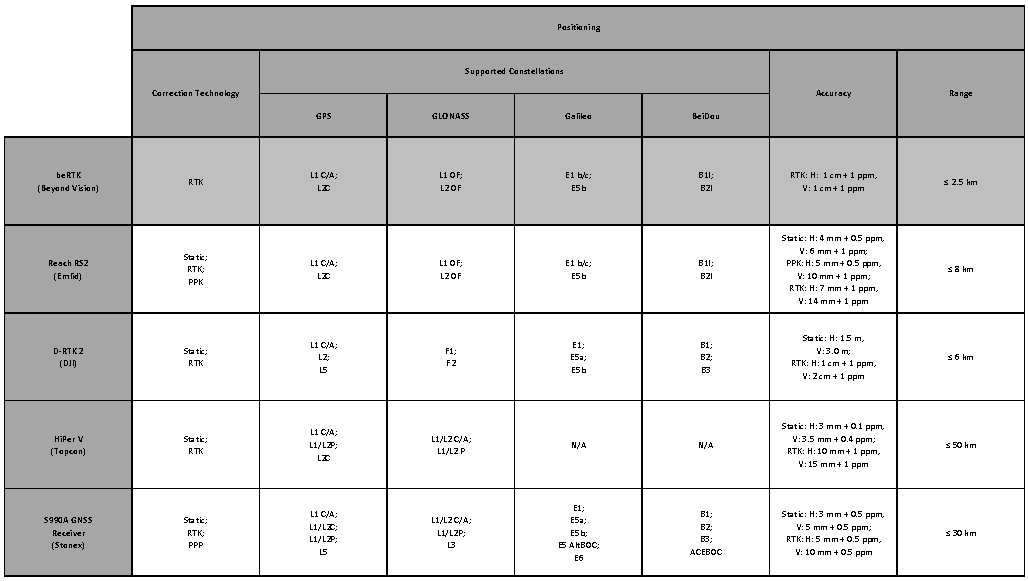
\includegraphics[width=1.0\textwidth]{Chapters/Figures/curr_solutions/POSITIONING_v2.pdf}
%     \caption{Some current base station solutions: positioning properties.}
% 	\label{fig:curr_sol_POSITIONING}
% \end{figure}

Looking at Table~\ref{tab:curr_sol_POSITIONING}, it is possible to see parameters referring to:
\begin{itemize}
    \item Correction Technology: Stating the positioning technologies supported by the device;
    \item Supported Constellations: Indicating the frequencies the device is able to work on, for each GNSS constellation;
    \item Accuracy: Presented for each positioning mode supported by the device, this parameter indicates the vertical and horizontal accuracy of the calculated position, expressing such with a small rate of error, known as PPM, which refers to a standardization of the error obtained in the observed measurement -- in millimeters per 1,000 meters, with respect to the orthometric height\footnote{Subtracting the geoid height from the ellipsoidal height results in the orthometric height; this height must be measured at an angle of 90$^{\circ}$ with respect to the \gls{geoid}.} (Figure~\ref{fig:orthometric_height}). It should be noted that, as stated in previous sections, standalone and post-processing positioning measurements result in a more accurate, comprehensive solution than is possible in real-time, hence the reduced error rates expected;
    \item Range: An estimation of the maximum baseline offered by the solution.
\end{itemize}
% meter imagem orthometric height
\begin{figure}[h]
    \centering
    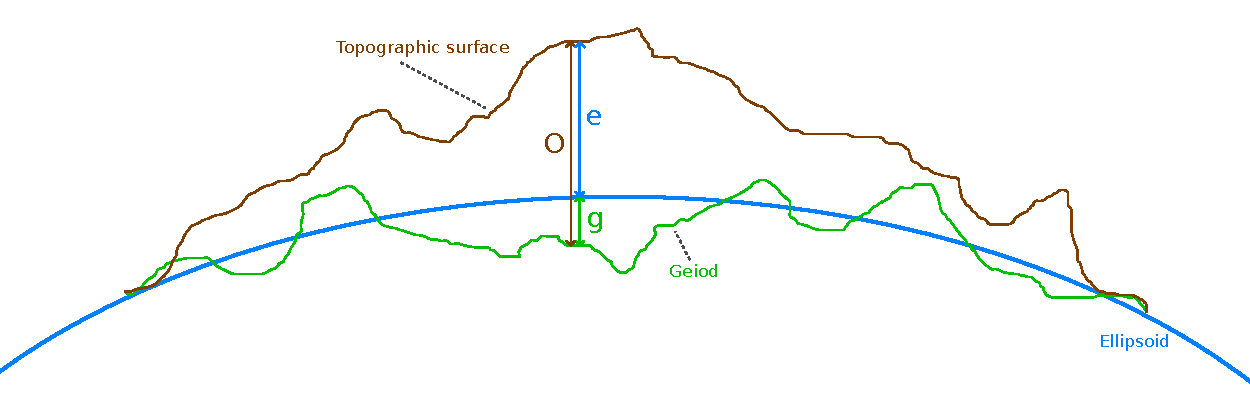
\includegraphics[width=0.95\textwidth]{Chapters/Figures/orthometric_height.pdf}
    \caption{Surfaces used for orthometric height calculation ($e=$ ellipsoidal height; $g=$ geoid height; $O=$ orthometric height).}
    \label{fig:orthometric_height}
\end{figure}

\begingroup
\begin{table}[h]
    \centering
	\captionsetup{justification=centering}
	\caption{Some current base station solutions: electrical properties.}
	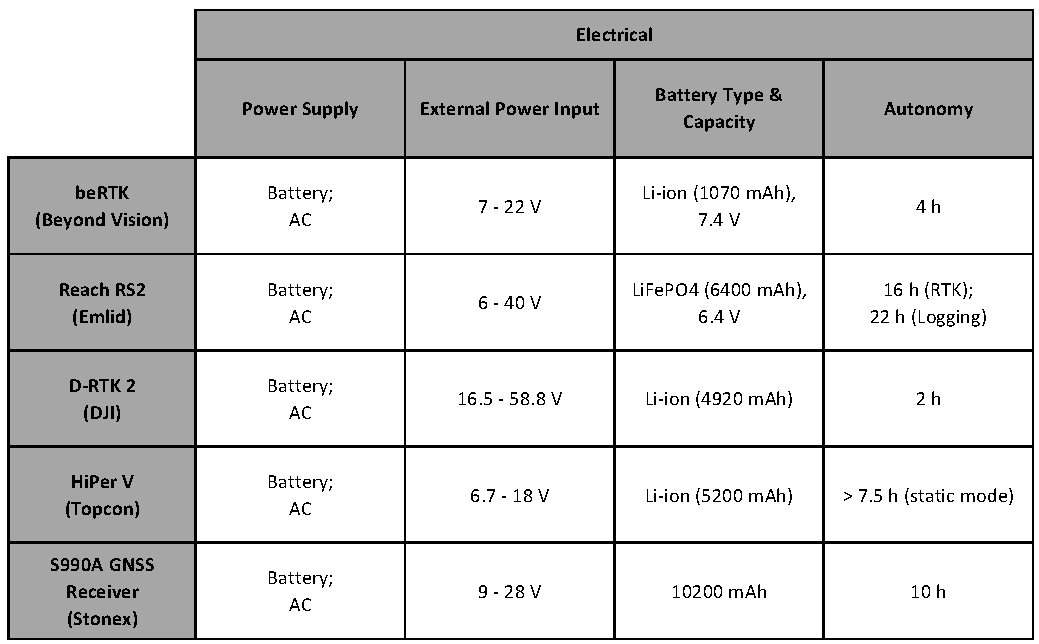
\includegraphics[width=1.0\textwidth]{Chapters/Figures/curr_solutions/ELECTRICAL_v2.pdf}
	\label{tab:curr_sol_ELECTRICAL}
\end{table}
\endgroup
% \begin{figure}[h]
% 	\centering
% 	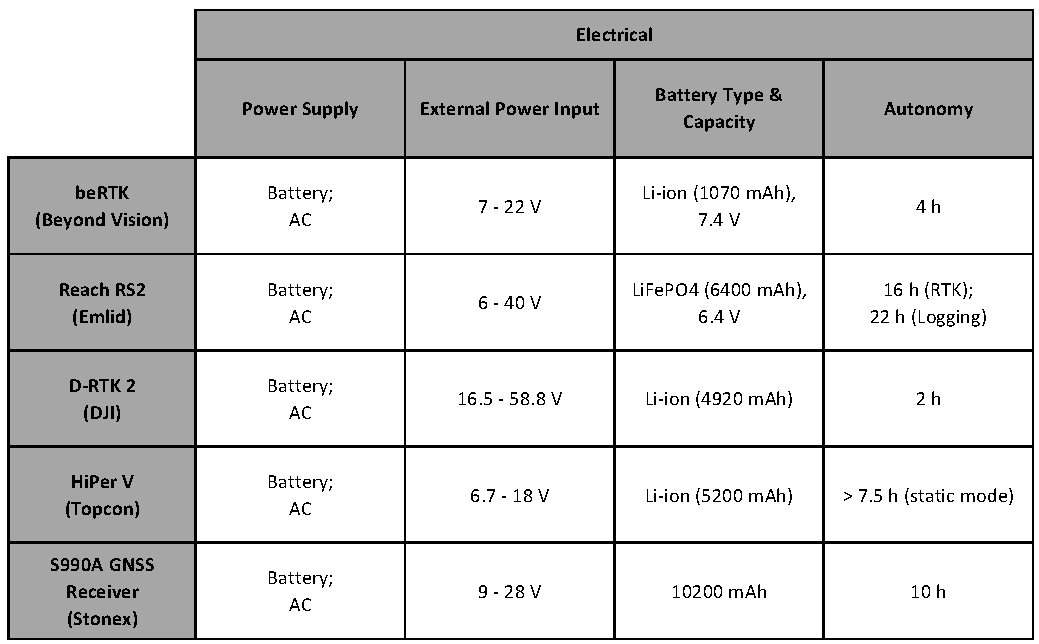
\includegraphics[width=1.0\textwidth]{Chapters/Figures/curr_solutions/ELECTRICAL_v2.pdf}
% 	\caption{Some current base station solutions: electrical properties.}
% 	\label{fig:curr_sol_ELECTRICAL}
% \end{figure}

Hardware-wise, Table~\ref{tab:curr_sol_ELECTRICAL} provides information about the devices' power and respective autonomy, which provides them with the ability to effectively make use of every communication protocol, as well as the types of data supported -- represented by Table~\ref{tab:curr_sol_CONNECTIONS}.

\begingroup
\begin{table}[h]
    \centering
	\captionsetup{justification=centering}
    \caption{Some current base station solutions: connectivity properties.}
	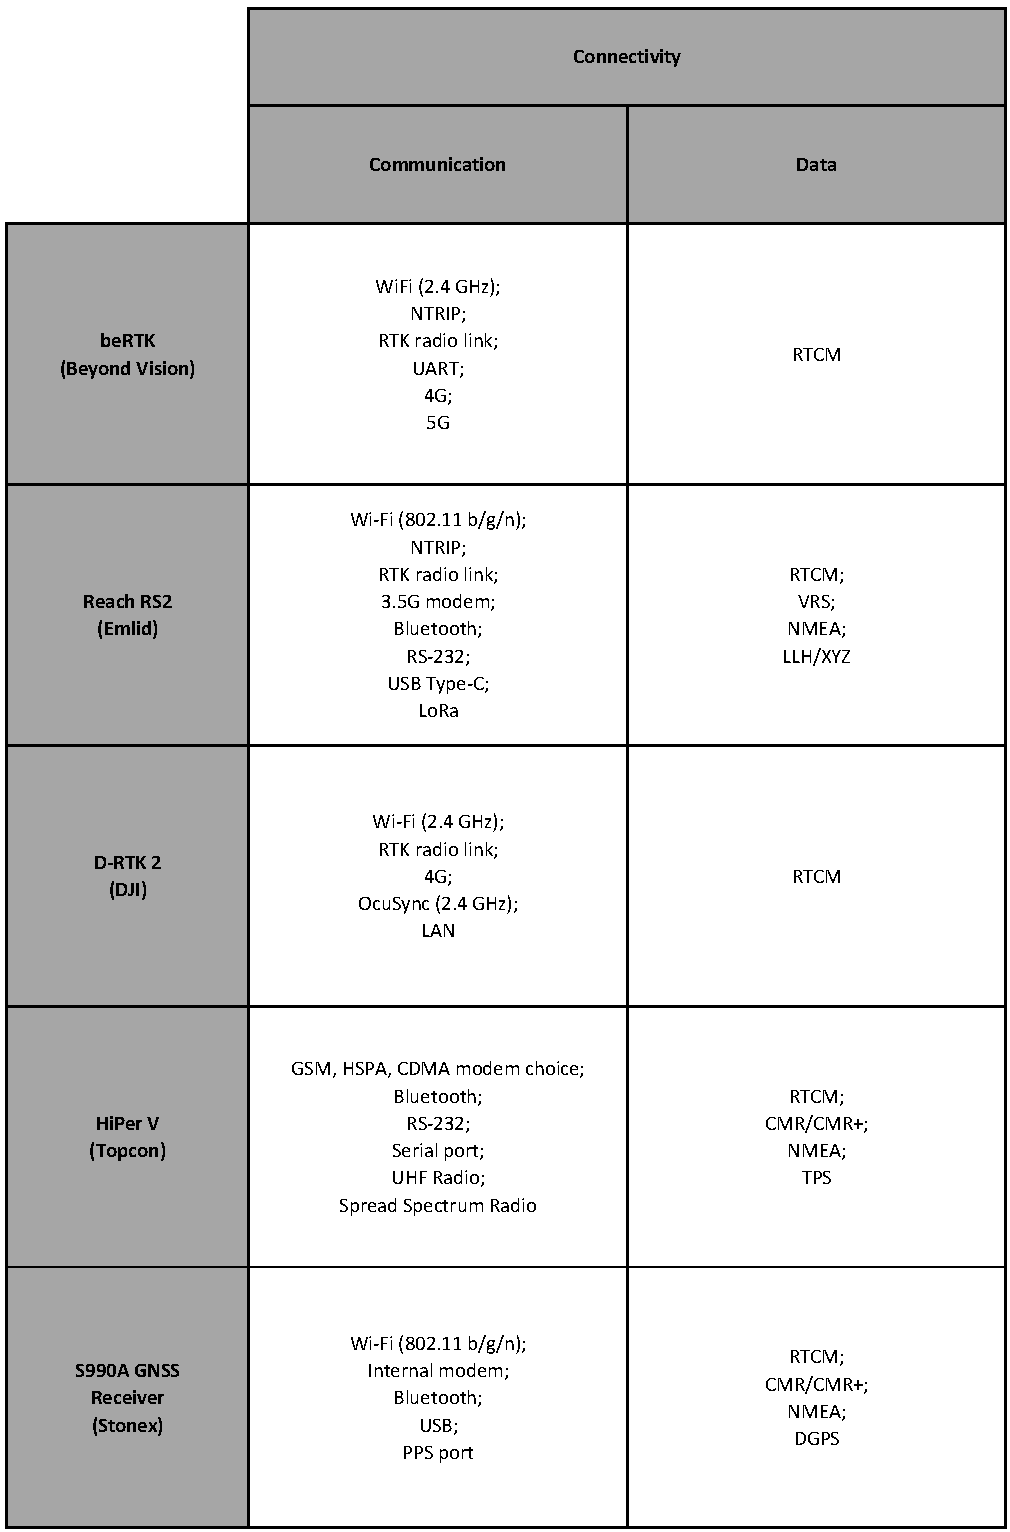
\includegraphics[width=0.8\textwidth]{Chapters/Figures/curr_solutions/CONNECTIONS_v2.pdf}
	\label{tab:curr_sol_CONNECTIONS}
\end{table}
\endgroup
% \begin{figure}[h]
% 	\centering
% 	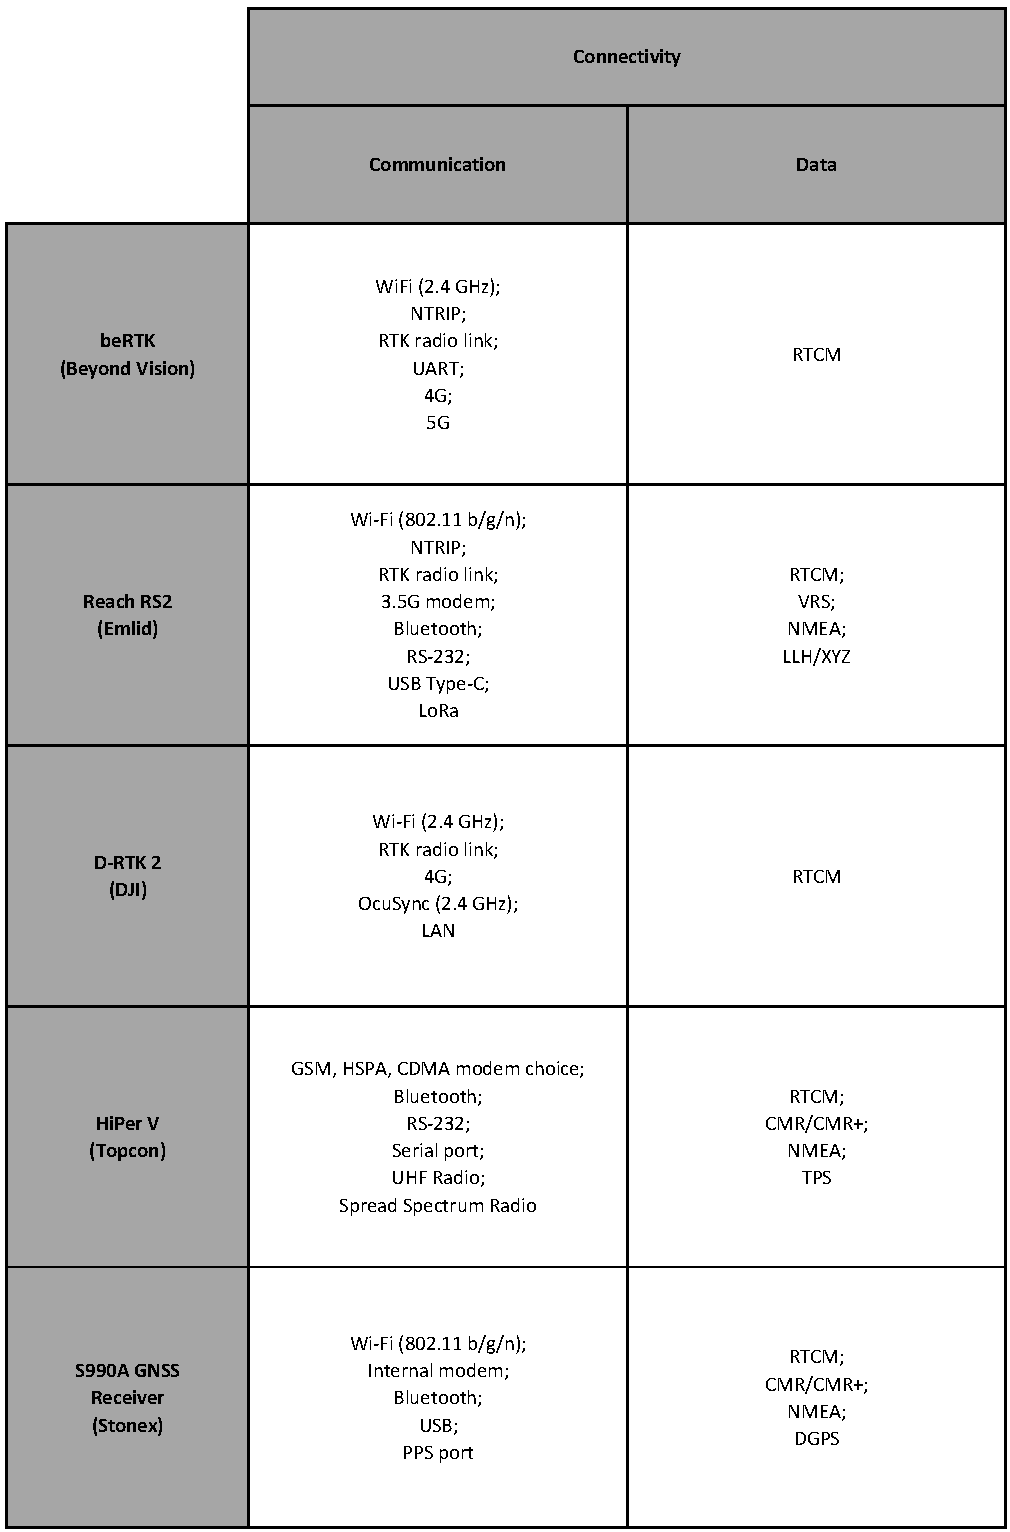
\includegraphics[width=0.8\textwidth]{Chapters/Figures/curr_solutions/CONNECTIONS_v2.pdf}
%     \caption{Some current base station solutions: connectivity properties.}
% 	\label{fig:curr_sol_CONNECTIONS}
% \end{figure}

Finally, shifting the focus to physical properties, Table~\ref{tab:curr_sol_MECH} informs about the devices' morphology and working conditions.

\begingroup
\begin{table}[H]
    \centering
	\captionsetup{justification=centering}
	\caption{Some current base station solutions: physical/mechanical properties.}
	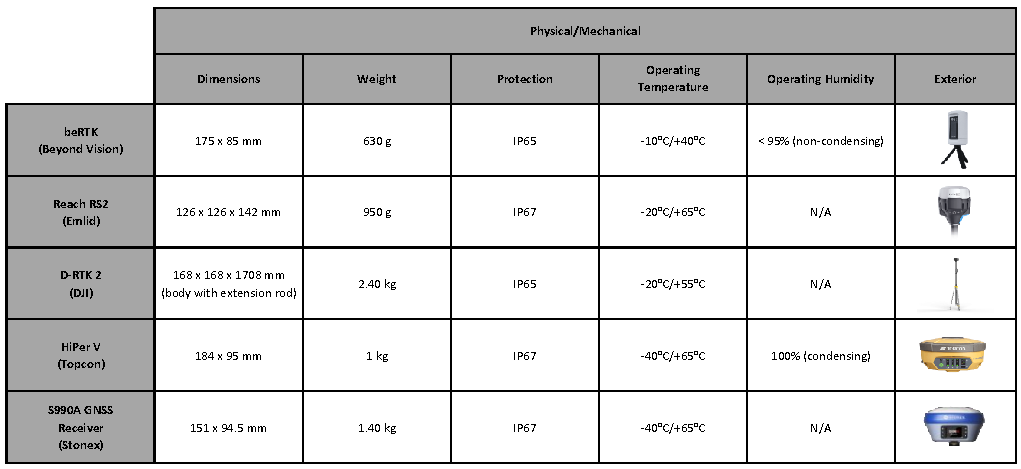
\includegraphics[width=1.0\textwidth]{Chapters/Figures/curr_solutions/MECH_v2.pdf}
	\label{tab:curr_sol_MECH}
\end{table}
\endgroup
% \begin{figure}[h]
% 	\centering
% 	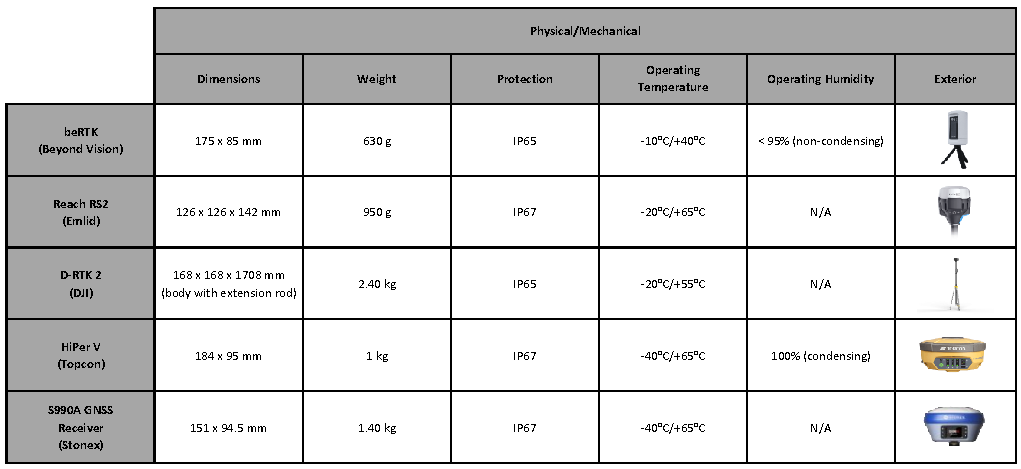
\includegraphics[width=1.0\textwidth]{Chapters/Figures/curr_solutions/MECH_v2.pdf}
% 	\caption{Some current base station solutions: physical/mechanical properties.}
% 	\label{fig:curr_sol_MECH}
% \end{figure}


% gravar como pdfs/imagem; meter no corpo do texto
% na versao final a tabela sera feita completamente em latex
\newpage
\subsection{Typical Architecture}\label{sec:II_architecture}

% qual é a arquitetura tipica deste tipo de equipamento?
% ao nivel da tecnologia, qual é o aspeto dos varios componentes do sistema?
    % base station, rover, links à net
    % ok, ja se sabem os integrantes de um sistema destes; vamos explicar como é constiutida uma base station por dentro - genericamente: chip, bateria, ...
All the properties presented in the previous section's tables should be treated as guidelines to the development of a new solution, which in turn needs to have a structured architecture.

% meter aqui o atual diagrama de blocos -- REDESENHAR E MUDAR TEXTO NOS BLOCOS
\begin{figure}[h]
	\centering
	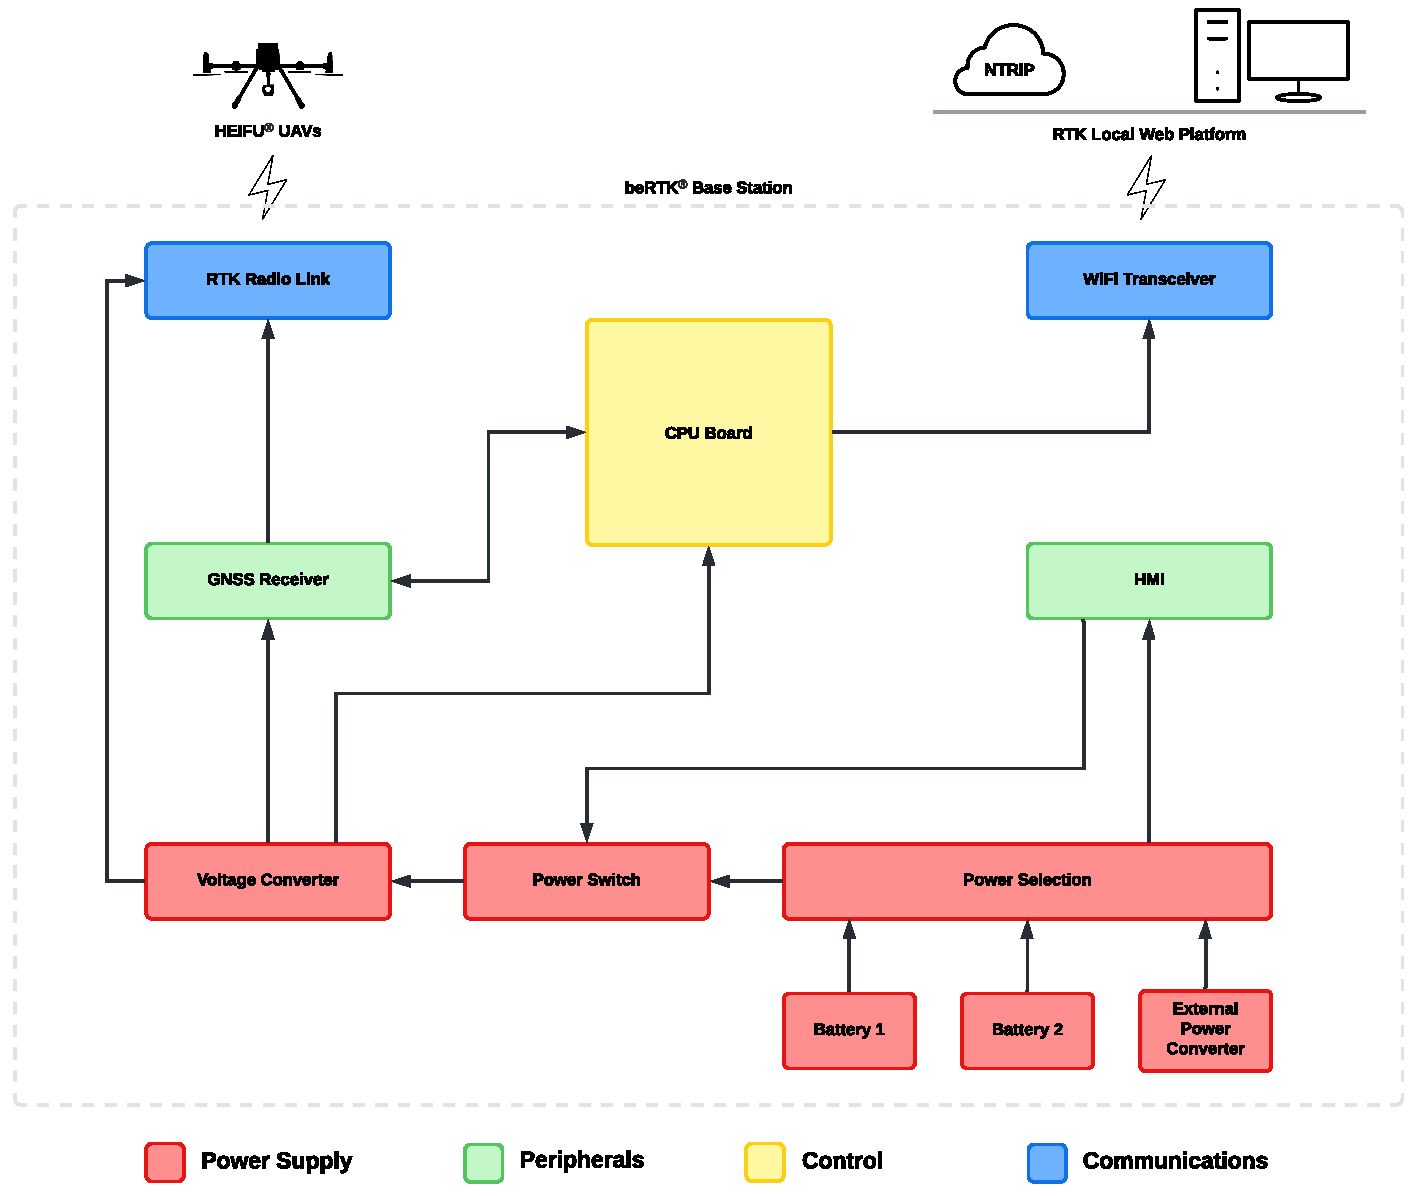
\includegraphics[width=1.0\textwidth]{Chapters/Figures/architecture_original_v2.pdf}
	\caption{beRTK\textsuperscript{\textregistered} Base Station's block diagram.}
	\label{fig:architecture_original}
\end{figure}

Figure~\ref{fig:architecture_original} presents a block diagram of the subsystems that make up Beyond Vision's current base station solution~\cite{beRTK_2022}.
The architecture introduces the system's division into four main subgroups:
\begin{itemize}
    \item Power Supply: Manages the device's power dynamics (i.e. power guidance, switch and conversion);
    \item Control: Commands the operation of the entire device; usually composed of microcontrollers;
    \item Peripherals: External units associated to device, in order to improve its operability. The \gls{HMI} seen is used to establish a connection between the user and the device itself. The GNSS Receiver performs the functions already described throughout this chapter;
    \item Communications: Used for connection to devices/networks, this group is in charge of establishing the links needed to complete the intended purpose of the device.
\end{itemize}

\subsubsection{Power Supply}\label{sec:II_architecture_PowerSupply}

beRTK\textsuperscript{\textregistered}'s architecture subgroups several major components which yield the characteristics presented in the previous tables. Starting with the Power Supply subgroup, the device must ensure the continuous and uninterrupted operation within its specified autonomy. Being that it is able to draw power either from an external adapter (i.e. from the power grid) or from DC batteries, there is a need for some tool able to select between differnt power supplies. Currently, and due to the baterries' characteristics (Table~\ref{tab:curr_sol_ELECTRICAL}), beRTK\textsuperscript{\textregistered} relies on a prioritized PowerPath\textsuperscript{\texttrademark} controller for such commutation, known as LTC4417. Defined by pin assignment, this controller selects the power input following a priority approach~\cite{LTC4417}; beRTK\textsuperscript{\textregistered}'s circuit prioritizes the external power converter first, followed by Battery 1 and then Battery 2.
%meter foto do esquematico

\subsubsection{Control}\label{sec:II_architecture_Control}

Skipping to the Control subgroup, i.e. the ``brains'' of the device, beRTK\textsuperscript{\textregistered} resorts to a computer, known as Raspberry Pi 4 Model B. This device is responsible for the reception and transmission of GNSS positions signals from the GNSS receiver, and is also tasked with the transmission of such signals to the Communications segment, all of this via its \gls{GPIO} pins~\cite{RPi4B}.
%meter foto do esquematico

\subsubsection{Peripherals}\label{sec:II_architecture_Peripherals}

Counting with a HMI, the Peripherals subgroup's GNSS receiver establishes a connection with all the other subgroups, and it is vital for the base station's purpose. beRTK\textsuperscript{\textregistered} uses a high precision multi-band GNSS module known as ZED-F9P, which enables centimeter level accuracy in just a few seconds. This professional receiver integrates RTK and GNSS technology, and its capability of supporting the four major GNSS constellations provides beRTK\textsuperscript{\textregistered} with the accuracy and range levels portrayed in Table~\ref{tab:curr_sol_POSITIONING}~\cite{ZED_F9P}.
%meter foto do esquematico

\subsubsection{Communications}\label{sec:II_architecture_Communications}

Finally, the Communications subgroup is responsible for establishing radio links with either an UAV device or an RTK local web platform. beRTK\textsuperscript{\textregistered} carries out the former link through the same GNSS receiver -- the ZED-F9P, while the latter link is formed via a Wi-Fi transceiver, known as a Digi XBee\textsuperscript{\textregistered} 3 RF Module, which employs the Zigbee specification to create a personal area network~\cite{XBee}, in order to retrieve positioning information from the internet.

% %% beyonddddddddddddddddddddddddddddddddddddddd:
% The main components of this diagram can be described as follows:
% -	RTK Local Web Platform: the RTK Base Station's Control Center. From this platform, the user can have full control over the Base Station. It is used in this context to retrieve the status of the RTK base Station and enable manual adjustments to its parameters;
% -	HEIFU™ Drone: The HEIFU™ drone is the mobile unit in the system. It uses the communication with this base station to improve its positioning accuracy;
% This document focuses on the RTK Base Station and as such, from this point on, only the blocks inside the RTK Base Station box will be considered. The blocks are described as follows:
% -	Battery1 and 2: Removable batteries to power the system in stand-alone mode;
% -	Power Selection Module: Logic module that selects from the different available power sources, the one that supplies the system at a given moment, being external power the main power source (highest priority). If external power is not available, the PSM first uses Battery1 and, when this battery is over, it uses Battery2 (lowest priority). Note that the power source will always switch to the highest priority power source that is considered valid based on its voltage.
% -	Power switch: A solid-state switch that ensures the capability of manually switching on and off the battery supply and so turning the RTK Base Station on and off respectively;
% -	CPU Board: The system's “brains”;
% -	RTK Positioning: Positioning module to accurately determine its position and transmit the correction signals;
% -	RTK Radio Link: Wireless link to the HEIFU™ drone to transmit the positioning information;
% -	Wi-Fi Transceiver: Wi-Fi link to connect to a user's personal computer.
% %%%%%%%%%%%%%%%%%%%%%%%%%%%%%%%%%%%%%%%%%%%%%%%%%%%%%%%%%%

The synergy from the association of each subgroup depends on the connections between them, which, on the other hand, will vary depending on the type of data transmission intended; different communication protocols that may fit better between each block are the reason behind that. Examples of this are the connections between the communication blocks (RTK Radio Link; Wi-Fi Transceiver) to UAVs manufactured by Beyond Vision -- HEIFU\textsuperscript{\textregistered} -- or to the RTK Local Web platform -- which subsequently connects to the network NTRIP --, which are performed using radiofrequency (a method already mentioned in this chapter).

\section{System Specifications and Requirements}\label{sec:II_Specs}

Aiming to implement a low-power solution for a new, improved version of the beRTK\textsuperscript{\textregistered} Base Station, the next step to take after gathering all the necessary knowledge on the subjects is to effectively define the system requirements.

For the development of a project, Beyond Vision's way of establishing its specifications is through a grammar table defined by codes in the following manner:

\begin{center}
	\textbf{<PROJ>.<SUBPROJ>.<SUBJECT>.<SERIAL>}
\end{center}
Where:
\begin{itemize}
	\item \textbf{<PROJ>}: Identifies the project. In this case it will be referred to as RTKBS;
	\item \textbf{<SUBPROJ>}: Identifies the subproject related to the specification;
	\item \textbf{<SUBJECT>}: Subgroups the specifications by area;
	\item \textbf{<SERIAL>}: Completes the individual specification with a unique ID number.
\end{itemize}

Therefore, the main requirements gathered for the project to develop are presented in Tables~\ref{tab:CRT_requirements}-\ref{tab:SW_requirements}, in the following sections.

\clearpage
\subsection{Certification Requirements}\label{sec:II_CRT_requirements}

This section describes the main certification requirements of the device.

\begingroup
\begin{table}[H]
	\captionsetup{justification=centering}
    \caption{beRTK\textsuperscript{\textregistered} Base Station certification requirements.}
	\label{tab:CRT_requirements}
	\centering

	% mini tabela: 1, 2, 3
	\begin{tabular}{rl}
        \toprule
		\textbf{RTKBS.MAIN.CRT.010} 			& \textbf{European Regulatory Framework} \\
		\multirow{2}*{}							& The RTK Base Station shall respect the current European \\
												& regulatory framework. \\
		\midrule
		\multirow{1}*{\textbf{Remarks:}}   & \\
		\bottomrule
		&\\
		&\\
		\toprule
		\textbf{RTKBS.MAIN.CRT.020} 		& \textbf{Electromagnetic Compatibility Certification} \\
		\multirow{2}*{}						& The RTK Base Station shall respect the current European \\
											& EMC (Electromagnetic Compatibility) standards. \\
		\midrule
		\multirow{2}*{\textbf{Remarks:}} 	& \emph{It must follow the European norms ETSI EN301 489-1,} \\
							  				& \emph{EN301 489-3 and EN301489-17.}\\
		\bottomrule
		&\\
		&\\
        \toprule
		\textbf{RTKBS.MAIN.CRT.030} 		& \textbf{Radio Equipment Certification} \\
		\multirow{4}*{}						& The RTK Base Station shall respect the current European \\
											& Radio Equipment Directive (RED), either by running \\
											& tests or by ensuring that all the radio equipment \\
											& on-board is already certified by its manufacturer. \\
		\midrule
		\multirow{4}*{\textbf{Remarks:}} 	& \emph{The list of RED related standards to be respected is} \\
							  				& \emph{at least (but not restricted to) the following:} \\
											& \emph{EN300 328:2015 (Wi-Fi); EN300 440 (Wi-Fi, ZigBee,} \\
											& \emph{Bluetooth); EN303 413 (GPS, RTK).}\\
		\bottomrule
	\end{tabular}
\end{table}
\endgroup
\clearpage
\subsection{Environmental Requirements}\label{sec:II_ENV_requirements}

This section describes the main environmental requirements of the device.

\begingroup
\begin{table}[H]
	\captionsetup{justification=centering}
    \caption{beRTK\textsuperscript{\textregistered} Base Station environmental requirements.}
	\label{tab:ENV_requirements}
	\centering

	% mini tabela: 4, 5
	\begin{tabular}{rl}
        \toprule
		\textbf{RTKBS.MAIN.ENV.010} 			& \textbf{Waste Management Certification} \\
		\multirow{3}*{}							& The RTK Base Station shall respect the current European \\
												& relating to WEEE (Waste of Electric and Electronic \\
												& Equipment). \\
		\midrule
		\multirow{3}*{\textbf{Remarks:}}   		& \emph{It must follow the following directives: 2012/19/EU} \\
												& \emph{(WEEE); 2006/66/EC (Battery recycling); 2011/65/EC} \\
												& \emph{(RoHS).} \\
		\bottomrule
		&\\
		&\\
        \toprule
		\textbf{RTKBS.MAIN.ENV.020} 		& \textbf{IP Protection} \\
		\multirow{2}*{}						& The RTK Base Station shall have an IP environmental \\
											& protection degree of IP65. \\
		\midrule
		\multirow{1}*{\textbf{Remarks:}} 	& \emph{Following European standard EN60529.} \\
		\bottomrule
	\end{tabular}
\end{table}
\endgroup

\subsection{Installation Requirements}\label{sec:II_INST_requirements}

This section describes the main installation requirements of the device.

\begingroup
\begin{table}[H]
	\captionsetup{justification=centering}
    \caption{beRTK\textsuperscript{\textregistered} Base Station installation requirements.}
	\label{tab:INST_requirements}
	\centering

	% mini tabela: 6
	\begin{tabular}{rl}
        \toprule
		\textbf{RTKBS.MAIN.INST.010} 			& \textbf{Easiness of Field Deploy} \\
		\multirow{4}*{}							& It shall be easy and fast to deploy the RTK base \\
												& Station on the field. Namely, it should only be needed \\
												& to choose a place, place the module, and turn the \\
												& module on.\\
												
		\midrule
		\multirow{1}*{\textbf{Remarks:}}   		& \\
		\bottomrule
	\end{tabular}
\end{table}
\endgroup
\clearpage
\subsection{Functional Requirements}\label{sec:II_FCT_requirements}

This section describes the main functional requirements of the device.

\begingroup
\begin{table}[H]
	\captionsetup{justification=centering}
    \caption{beRTK\textsuperscript{\textregistered} Base Station functional requirements.}
	\label{tab:FCT_requirements}
	\centering

	% mini tabela: 7, 8, 9, 10, 11
	\begin{tabular}{rl}
        \toprule
		\textbf{RTKBS.MAIN.FCT.010} 			& \textbf{RTK Base} \\
		\multirow{5}*{}							& As an RTK Base Station, the main purpose of this device \\
												& is to accurately calculate its position. It shall also \\
												& transmit the position wirelessly to the devices around \\
												& that are capable of receiving and processing this \\
												& information. \\
		\midrule
		\multirow{1}*{\textbf{Remarks:}}   & \\
		\bottomrule
		&\\
		&\\
		\toprule
		\textbf{RTKBS.MAIN.FCT.020} 		& \textbf{Positioning Error} \\
		\multirow{2}*{}						& The RTK Base Station shall achieve a positioning error \\
											& of less than 2 cm. \\
		\midrule
		\multirow{2}*{\textbf{Remarks:}} 	& \emph{The u-Blox module ZED-F9P should be the basis for} \\
							  				& \emph{this RTK system.}\\
		\bottomrule
		&\\
		&\\
        \toprule
		\textbf{RTKBS.MAIN.FCT.030} 		& \textbf{On-board Intelligence} \\
		\multirow{4}*{}						& The RTK Base Station shall have a control unit, able to \\
											& carry out a pre-determined set of instructions, accept \\
											& instructions in real-time, receive NTRIP information \\
											& and send correction signals to the HEIFU\textsuperscript{\textregistered} UAV. \\
		\midrule
		\multirow{1}*{\textbf{Remarks:}} 	& \\
		\bottomrule
		&\\
		&\\
        \toprule
		\textbf{RTKBS.MAIN.FCT.040} 		& \textbf{Wireless Link} \\
		\multirow{4}*{}						& The RTK Base Station shall be able to wirelessly \\
											& transmit the differential correction information to the \\
											& devices around. \\
		\midrule
		\multirow{1}*{\textbf{Remarks:}} 	& \\
		\bottomrule
		&\\
		&\\
        \toprule
		\textbf{RTKBS.MAIN.FCT.050} 		& \textbf{Wireless Link Range} \\
		\multirow{1}*{}						& The wireless link shall reach at least 1 km VLOS. \\
		\midrule
		\multirow{1}*{\textbf{Remarks:}} 	& \\
		\bottomrule
	\end{tabular}
\end{table}
\endgroup
\clearpage
\subsection{Mechanical Requirements}\label{sec:II_MEC_requirements}

This section describes the main mechanical requirements of the device.

\begingroup
\begin{table}[H]
	\captionsetup{justification=centering}
    \caption{beRTK\textsuperscript{\textregistered} Base Station mechanical requirements.}
	\label{tab:MEC_requirements}
	\centering

	% mini tabela: 12, 13, 14
	\begin{tabular}{rl}
        \toprule
	    \textbf{RTKBS.MAIN.MEC.010} 		& \textbf{Enclosure} \\
	    \multirow{5}*{}						& The RTK Base Station shall count on a plastic enclosure \\
											& as a shelter from the environment. This enclosure should \\
											& be designed in a way that is does not interfere with the \\
											& radio signals needed for its operation (namely \\
											& positioning and wireless communications).\\
		\midrule
		\multirow{1}*{\textbf{Remarks:}}   & \\
		\bottomrule
		&\\
		&\\
		\toprule
		\textbf{RTKBS.MAIN.MEC.020} 		& \textbf{Tripod Attachment} \\
		\multirow{3}*{}						& The RTK Base Station's enclosure shall be designed in \\
											& order to be possible to attach it to the top of a tripod \\
											& with a 5/8'' screw. \\
		\midrule
		\multirow{1}*{\textbf{Remarks:}} 	& \\
		\bottomrule
		&\\
		&\\
        \toprule
		\textbf{RTKBS.MAIN.MEC.030} 		& \textbf{Minimize Connectors} \\
		\multirow{3}*{}						& The RTK Base Station shall be designed so to minimize\\
											& the number of connectors to the outside world. This \\
											& includes antennae. \\
		\multirow{3}*{\textbf{Remarks:}}    & \emph{The idea is to ease and accelerate the deployment on the}\\
											& \emph{field, as well as minimize the vulnerability to}\\
											& \emph{external parameters.} \\
		\bottomrule
	\end{tabular}
\end{table}
\endgroup
\clearpage
\subsection{Electrical Requirements}\label{sec:II_PWS_requirements}

This section describes the main electrical requirements of the device.

\begingroup
\begin{table}[H]
	\captionsetup{justification=centering}
    \caption{beRTK\textsuperscript{\textregistered} Base Station electrical requirements.}
	\label{tab:PWS_requirements}
	\centering

	% mini tabela: 15, 16, 17, 18, 19
	\begin{tabular}{rl}
        \toprule
		\textbf{RTKBS.MAIN.PWS.010} 			& \textbf{Main Power Supply} \\
		\multirow{6}*{}							& The RTK Base Station shall run on electricity, being \\
												& the main power source a connection to an external power \\
												& supply. It shall accept voltages between +7 VDC and \\
												& +22 VDC, enabling the connection to a standard solar \\
												& panel, a car battery or a mains power supply capable of \\
												& delivering a voltage within that range. \\
		\midrule
		\multirow{1}*{\textbf{Remarks:}}   & \\
		\bottomrule
		&\\
		&\\
		\toprule
		\textbf{RTKBS.MAIN.PWS.020} 		& \textbf{Battery} \\
		\multirow{4}*{}						& The RTK Base Station shall count on a single battery, \\
											& enabling it to be used on the field where a mains power \\
											& connection is not available. This battery shall be \\
											& embedded on the device's electronic system. \\
		\midrule
		\multirow{1}*{\textbf{Remarks:}} 	& \\
		\bottomrule
		&\\
		&\\
        \toprule
		\textbf{RTKBS.MAIN.PWS.030} 		& \textbf{Power Supply Switching} \\
		\multirow{5}*{}						& Having two separate power sources, the RTK Base Station \\
											& shall prioritize external power input, switching to the \\
											& internal battery when that connection cannot be \\
											& established. This transition must be smooth in order to \\
											& ensure continuous operation. \\
		\midrule
		\multirow{1}*{\textbf{Remarks:}} 	& \\
		\bottomrule
		&\\
		&\\
        \toprule
		\textbf{RTKBS.MAIN.PWS.040} 		& \textbf{Power Consumption} \\
		\multirow{3}*{}						& The RTK Base Station shall not exceed an average of \\
											& 400 mA of current consumption at 5 VDC voltage level. \\
											& That is, it shall not exceed a power consumption of 2 W.\\
		\midrule
		\multirow{1}*{\textbf{Remarks:}} 	& \\
		\bottomrule
		&\\
		&\\
        \toprule
		\textbf{RTKBS.MAIN.PWS.050} 		& \textbf{Power Switch} \\
		\multirow{3}*{}						& It shall be possible to turn the RTK Base Station on and\\
											& off by means of a pushbutton switch in toggle mode. This \\
											& button shall be externally available to the user. \\
		\midrule
		\multirow{1}*{\textbf{Remarks:}} 	& \\
		\bottomrule
	\end{tabular}
\end{table}
\endgroup
\clearpage
\subsection{Communication Requirements}\label{sec:II_COM_requirements}

This section describes the main communication requirements of the device.

\begingroup
\begin{table}[H]
	\captionsetup{justification=centering}
    \caption{beRTK\textsuperscript{\textregistered} Base Station communication requirements.}
	\label{tab:COM_requirements}
	\centering

	% mini tabela: 20, 21, 22
	\begin{tabular}{rl}
        \toprule
		\textbf{RTKBS.MAIN.COM.010} 			& \textbf{Communication with NTRIP Platform} \\
		\multirow{3}*{}							& The RTK Base Station shall be capable of establishing \\
												& communications with an NTRIP platform by using a \\
												& Wi-Fi radio link. \\
		\midrule
		\multirow{1}*{\textbf{Remarks:}}   & \\
		\bottomrule
		&\\
		&\\
		\toprule
		\textbf{RTKBS.MAIN.COM.020} 		& \textbf{Communication with the UAVs} \\
		\multirow{3}*{}						& The RTK Base Station shall be capable of establishing \\
											& wireless communications with the UAVs by using a \\
											& well-established local communication radio protocol. \\
		\midrule
		\multirow{2}*{\textbf{Remarks:}} 	& \emph{Communication can be established either using the} \\
											& \emph{IEEE 802.15.4 or LoRa protocols.}\\
		\bottomrule
		&\\
		&\\
        \toprule
		\textbf{RTKBS.MAIN.COM.030} 		& \textbf{Communication with the User's Computer} \\
		\multirow{3}*{}						& The RTK Base Station shall be capable of establishing \\
											& communications with an external computer by using a \\
											& Wi-Fi radio link. \\
		\midrule
		\multirow{1}*{\textbf{Remarks:}} 	& \\
		\bottomrule
	\end{tabular}
\end{table}
\endgroup
\clearpage
\subsection{User Interface Requirements}\label{sec:II_HMI_requirements}

This section describes the main user interface requirements of the device.

\begingroup
\begin{table}[H]
	\captionsetup{justification=centering}
    \caption{beRTK\textsuperscript{\textregistered} Base Station user interface requirements.}
	\label{tab:HMI_requirements}
	\centering

	% mini tabela: 23, 24, 25, 26
	\begin{tabular}{rl}
        \toprule
		\textbf{RTKBS.MAIN.HMI.010} 			& \textbf{Power Button} \\
		\multirow{2}*{}							& The RTK Base Station shall exhibit, on its front panel, \\
												& the power button. \\
		\midrule
		\multirow{1}*{\textbf{Remarks:}}   & \\
		\bottomrule
		&\\
		&\\
		\toprule
		\textbf{RTKBS.MAIN.HMI.020} 		& \textbf{Battery Status} \\
		\multirow{3}*{}						& The RTK Base Station shall exhibit, on its front panel, \\
											& the status of the power source currently being used, by \\
											& means of four blue LEDs. \\
		\midrule
		\multirow{1}*{\textbf{Remarks:}} 	& \\
		\bottomrule
		&\\
		&\\
        \toprule
		\textbf{RTKBS.MAIN.HMI.030} 		& \textbf{Power Source Indication} \\
		\multirow{3}*{}						& The RTK Base Station shall exhibit, on its front panel, \\
											& an indication of which power sources are available, by \\
											& means of three blue LEDs. \\
		\midrule
		\multirow{1}*{\textbf{Remarks:}} 	& \\
		\bottomrule
		&\\
		&\\
        \toprule
		\textbf{RTKBS.MAIN.HMI.040} 		& \textbf{Power Connector} \\
		\multirow{3}*{}						& The RTK Base Station shall exhibit, on its back panel, \\
											& one connector enabling the connection to an external \\
											& power source. \\
		\midrule
		\multirow{1}*{\textbf{Remarks:}} 	& \\
		\bottomrule
	\end{tabular}
\end{table}
\endgroup
\clearpage
\subsection{Software Requirements}\label{sec:II_SW_requirements}

This section describes the main software requirements of the device.

\begingroup
\begin{table}[H]
	\captionsetup{justification=centering}
    \caption{beRTK\textsuperscript{\textregistered} Base Station software requirements.}
	\label{tab:SW_requirements}
	\centering

	% mini tabela: 27, 28, 29, 30
	\begin{tabular}{rl}
        \toprule
		\textbf{RTKBS.MAIN.SW.010} 				& \textbf{Operating system} \\
		\multirow{2}*{}							& The RTK Base Station's control unit shall be able to \\
												& run an embedded operating system. \\
		\midrule
		\multirow{1}*{\textbf{Remarks:}}   & \\
		\bottomrule
		&\\
		&\\
		\toprule
		\textbf{RTKBS.MAIN.SW.020} 			& \textbf{RTK Local Web Platform} \\
		\multirow{2}*{}						& The RTK Base Station's control unit shall have a \\
											& Local Web Platform that controls the RTK function. \\
		\midrule
		\multirow{1}*{\textbf{Remarks:}} 	& \\
		\bottomrule
		&\\
		&\\
        \toprule
		\textbf{RTKBS.MAIN.SW.030} 			& \textbf{Configuration} \\
		\multirow{4}*{}						& The RTK base Station shall include a configuration \\
											& interface, enabling a user to configure the base \\
											& parameters. This interface shall be available via the \\
											& RTK Local Web Platform. \\
		\midrule
		\multirow{1}*{\textbf{Remarks:}} 	& \\
		\bottomrule
		&\\
		&\\
        \toprule
		\textbf{RTKBS.MAIN.SW.040} 			& \textbf{Logs} \\
		\multirow{3}*{}						& The RTK base Station shall record the main activities \\
											& in a log file, so it can be possible to back trace its \\
											& behaviour. \\
		\midrule
		\multirow{1}*{\textbf{Remarks:}} 	& \\
		\bottomrule
	\end{tabular}
\end{table}
\endgroup
